This chapter compares a suite of weak lensing statistics obtained from two simulation sets: BIGBOX and TILED. Our goal is to quantify differences in mean values, covariance, and correlation matrices to evaluate the impacts of super-sample covariance and other systematic effects on these measurements. We will also examine the effects of shape noise, smoothing scales, and box replication artifacts on the results. Unless otherwise specified, the main results presented are derived from noiseless simulations with a smoothing scale of 2 arcminutes. Additionally, $C_\ell$ and bispectrum results are normalized by factors of $\ell(\ell+1)/2\pi$ and $\ell^4$, respectively.

\section{Comparison of Mean and Variance for summary statistics}
We analyze and compare the mean ($\mu$) and variance ($\sigma^2$) of summary statistics derived from the BIGBOX and TILED simulations. Figures~\ref{fig:ell_main} and~\ref{fig:nu_main} illustrate these comparisons for the angular power spectrum, bispectrum, and other higher-order statistics, highlighting the differences caused by simulation methodologies and super-sample covariance effects.

The mean values, represented by the ratio $R_{\mu}$, exhibit remarkable consistency in capturing statistical distributions across the two simulation sets. For most summary statistics, deviations in $R_{\mu}$ are less than $1\%$, underscoring the robustness of both pipelines in reproducing the underlying statistics. By comparing with theoretical predictions, there are no severe conflicts between the theory and the simulations.

However, systematic deviations between TILED and BIGBOX emerge at low $\nu$ values for peak counts, minima, and Minkowski Functionals and at high $nu$ values for minima (left panels in Figure~\ref{fig:nu_main}). These deviations likely stem from the limited ability of the TILED simulations to resolve super high-density and low-density regions, leading to fewer data points in the extreme tails of the distribution.

In contrast, the variance ratios $R_{\sigma^2}$ reveal more pronounced differences, highlighting the critical impact of super-sample covariance on variance measurements. The variance for the angular power spectrum (top-right panel in Figure~\ref{fig:ell_main}) exhibits a significant increase in the BIGBOX simulations at high $\ell$, consistent with the expected amplification due to the inclusion of larger-scale modes in the BIGBOX setup, which are absent in the TILED simulations. Furthermore, variance ratio discrepancies grow with increasing source redshift, reflecting the progressive loss of large-scale modes in the TILED simulations. For $\nu$-binned statistics (right panels in Figure~\ref{fig:nu_main}), the BIGBOX simulations consistently yield higher variances across nearly all $\nu$ bins, with this trend becoming more pronounced at higher source redshifts. %This behavior is opposite to that observed in \citet{Sato_2009}

\begin{figure}[ht]
    \centering
    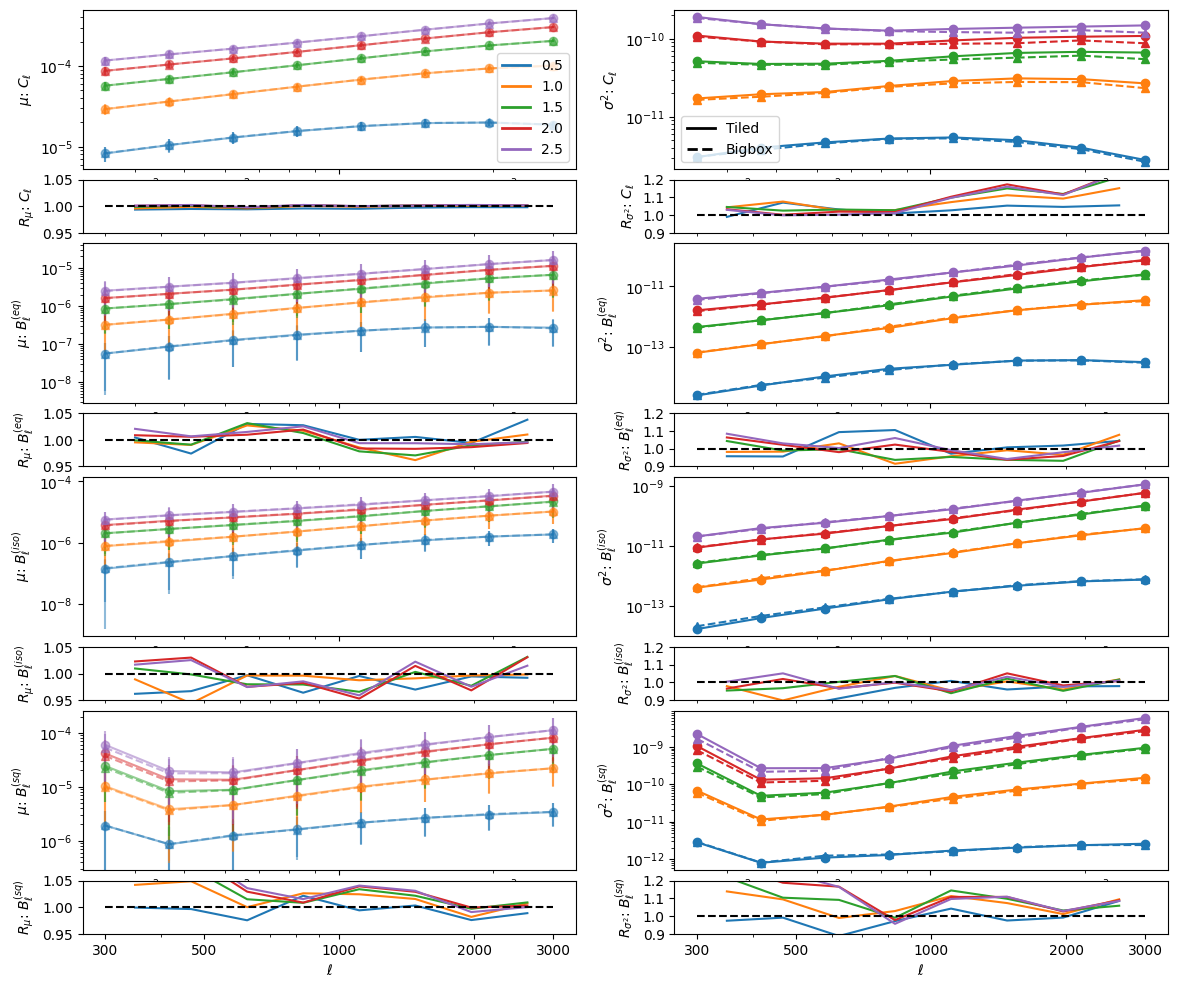
\includegraphics[width=\textwidth]{figures/results/ell_main.png}
    \caption[Comparison of Mean and Variance for $C^{\kappa\kappa}_{\ell}$ and Bispectrum]
    {Comparison of the mean and variance for the angular power spectrum ($C^{\kappa\kappa}{\ell}$) and the bispectrum components across three configurations: equilateral ($B{\ell}^{(eq)}$), isosceles ($B_{\ell}^{(iso)}$), and squeezed ($B_{\ell}^{(sq)}$). Results are presented for the BIGBOX and TILED simulations across source redshifts $z_s = 0.5$, 1.0, 1.5, 2.0, and 2.5.}
    \label{fig:ell_main}
\end{figure}

\begin{figure}[p]
    \centering
    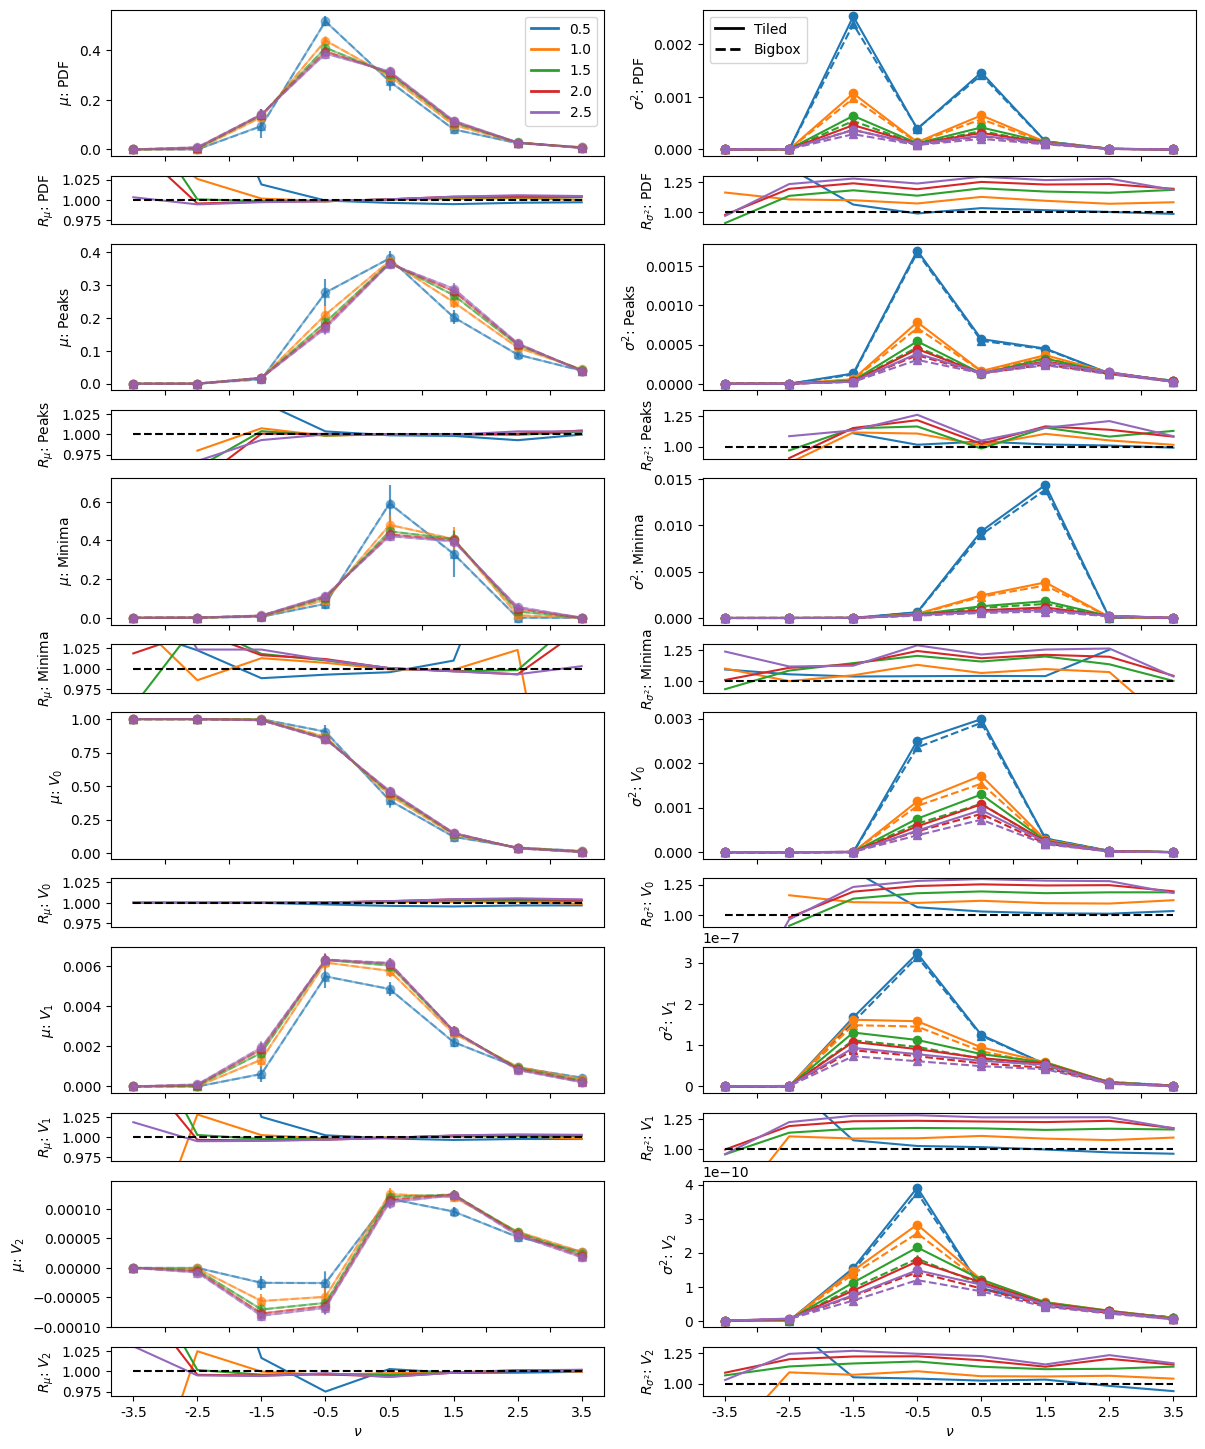
\includegraphics[width=\textwidth]{figures/results/nu_main.png}
    \caption[Comparison of Mean and Variance for Non-Correlation Statistics]
    {Comparison of the mean and variance for $\nu$-binned statistics, including the Minkowski Functionals ($V_0$, $V_1$, $V_2$), the probability density function (PDF), and peak and minima counts. Results are derived from the BIGBOX and TILED simulations across source redshifts $z_s = 0.5$, 1.0, 1.5, 2.0, and 2.5, highlighting their sensitivity to super-sample covariance.}
    \label{fig:nu_main}
\end{figure}

\clearpage

\section{Analysis of Covariance and Correlation Matrices}
To quantify the impact of super-sample covariance on the off-diagonal terms, we compare the covariance and correlation matrices of the summary statistics.

Figure~\ref{fig:cov_bigbox} presents the covariance matrices for the BIGBOX simulations. Figure~\ref{fig:cov_tiled} displays the corresponding matrices for the TILED simulations. The general covariance structures are consistent between the two simulation sets, with the BIGBOX simulations exhibiting higher covariance values on average. Figure~\ref{fig:corr_main} illustrates the correlation matrices for the BIGBOX and TILED simulations. The upper-left triangle of each panel shows the correlation coefficients derived from the BIGBOX simulations, while the lower-right triangle displays the corresponding values from the TILED simulations. No obvious discrepancies are visible in the color scale, suggesting that the correlation structures are almost consistent between the two simulation sets.

Figures~\ref{fig:cov_ratio_main} and~\ref{fig:corr_ratio_main} illustrate the ratios of covariance and correlation matrices between the BIGBOX and TILED simulations, denoted $R_{\text{Cov}}$ and $R_{\rho}$, respectively. These comparisons quantitatively assess the influence of super-sample covariance on the diagonal and off-diagonal elements of the covariance structure. The covariance ratios $R_{\text{Cov}}$ generally exceed unity, ranging from $10\%$ to $30\%$ above the baseline values for most summary statistics. This consistent elevation underscores the significant contribution of super-sample covariance to the overall covariance matrix. Conversely, the correlation ratios $R_{\rho}$ typically deviate by less than $5\%$. These results suggest that the super-sample effect impacts not only the diagonal terms but also the off-diagonal elements of the covariance matrix, thereby elevating the entire covariance structure. Notable exceptions to these trends occur in the angular power spectrum and peak/minima counts. For the angular power spectrum, larger deviations in the correlation ratios are consistent with super-sample covariance effects, which arise from the strong correlations introduced by shared large-scale modes, particularly at small $\ell$. In contrast, the deviations observed in the peak/minima counts likely stem from systematic shifts in peak positions within the TILED simulations, leading to changes in correlations near the peak bins. For a summary of the average ratios of covariance and correlation matrices, see Figure~\ref{fig:avg_main}.

\begin{figure}[ht]
    \begin{minipage}{0.48\textwidth}
        \centering
        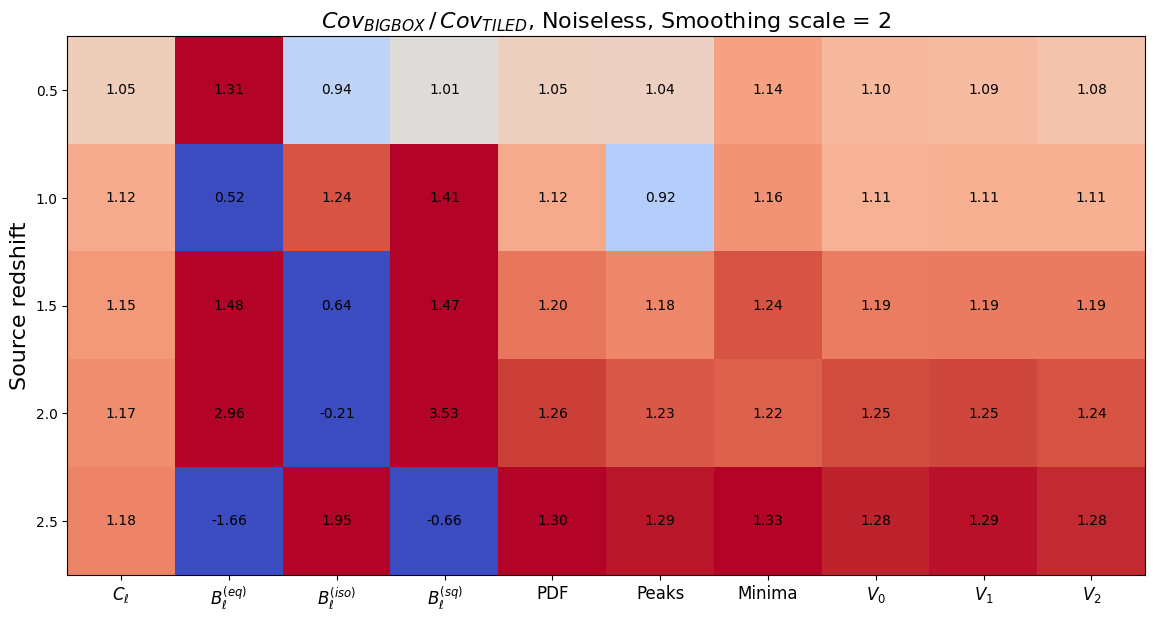
\includegraphics[width=\textwidth]{figures/results/avg_cov_ratio_main.png}
    \end{minipage}
    \begin{minipage}{0.48\textwidth}
        \centering
        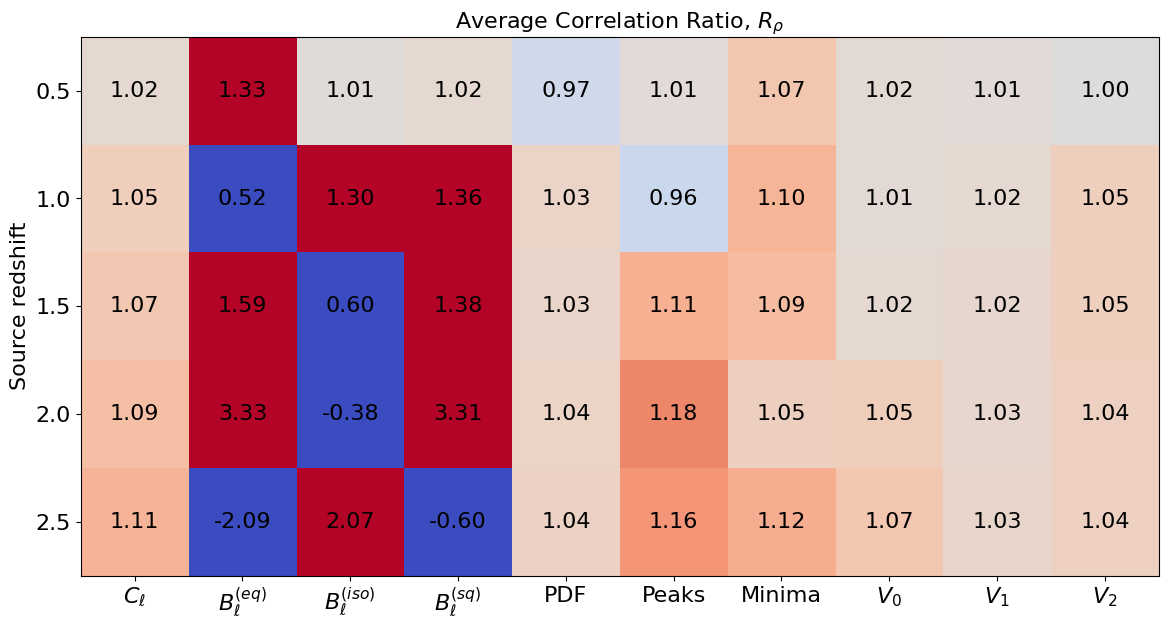
\includegraphics[width=\textwidth]{figures/results/avg_corr_ratio_main.png}
    \end{minipage}
    \caption[Average BIGBOX/TILED Ratios of Covariance and Correlation Matrices]{Average ratios of covariance matrices (left) and correlation matrices (right) between the BIGBOX and TILED simulations for multiple source redshifts. The increasing trend in the covariance ratios highlights the contribution of super-sample covariance to the covariance structure.}
    \label{fig:avg_main}
\end{figure}

\begin{figure}[p]
    \centering
    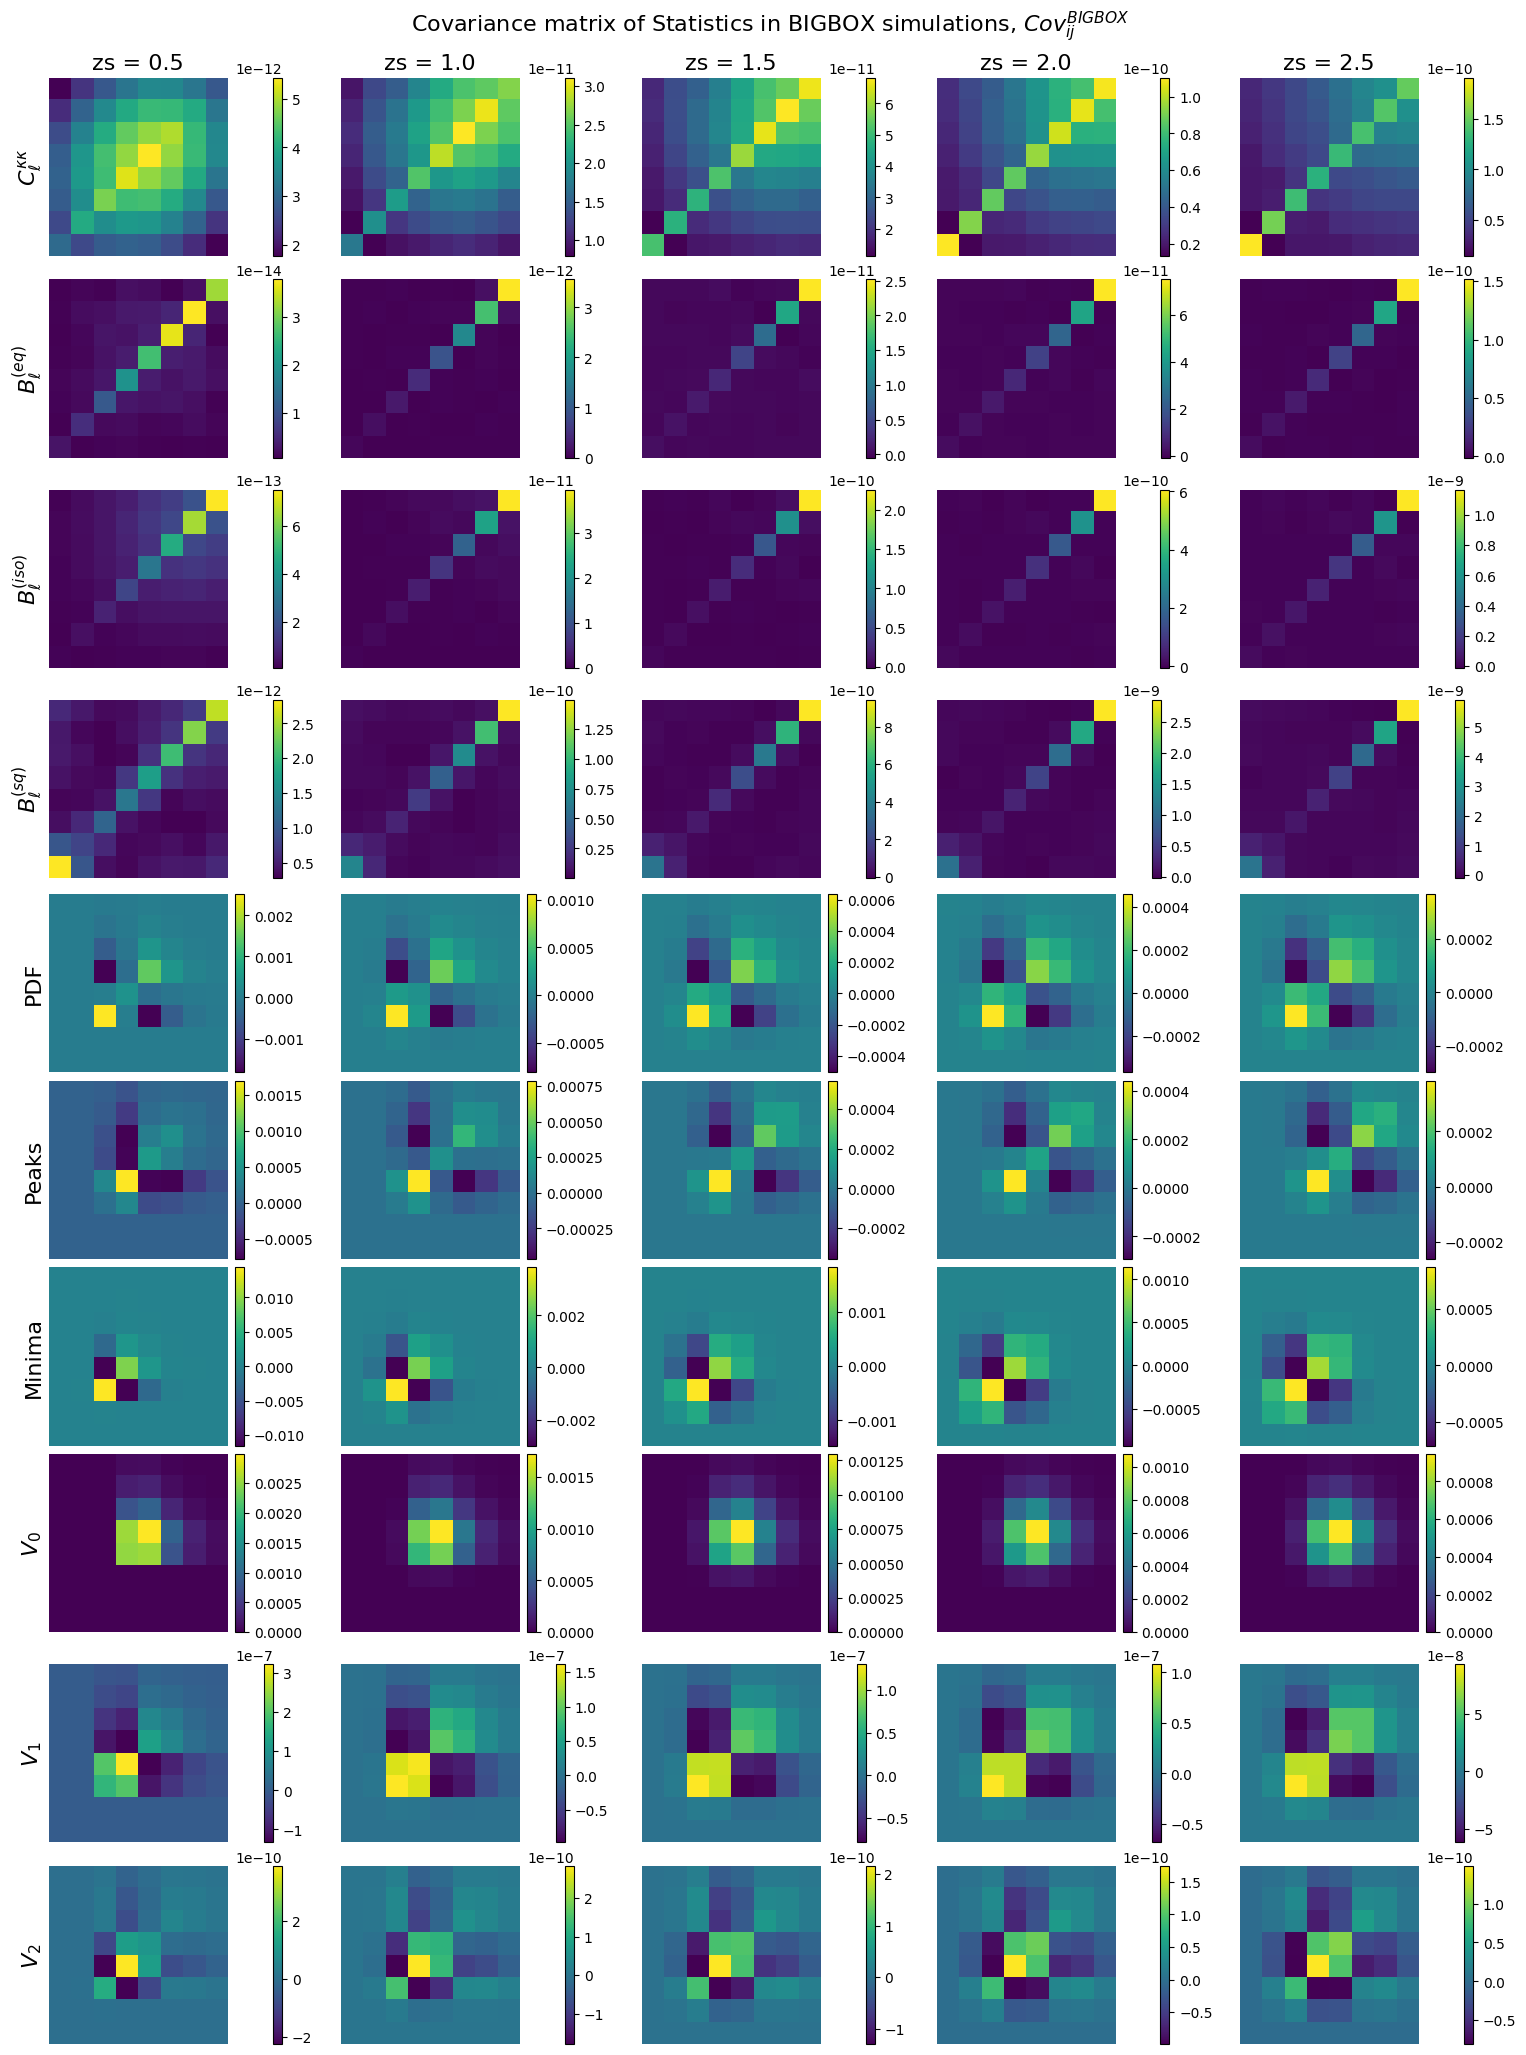
\includegraphics[width=\textwidth]{figures/results/cov_bigbox.png}
    \caption[Covariance Matrices of summary statistics in BIGBOX Simulations]{Covariance matrices of summary statistics in the BIGBOX simulations across multiple source redshifts, illustrating the covariance structure influenced by super-sample covariance.}
    \label{fig:cov_bigbox}
\end{figure}

\begin{figure}[p]
    \centering
    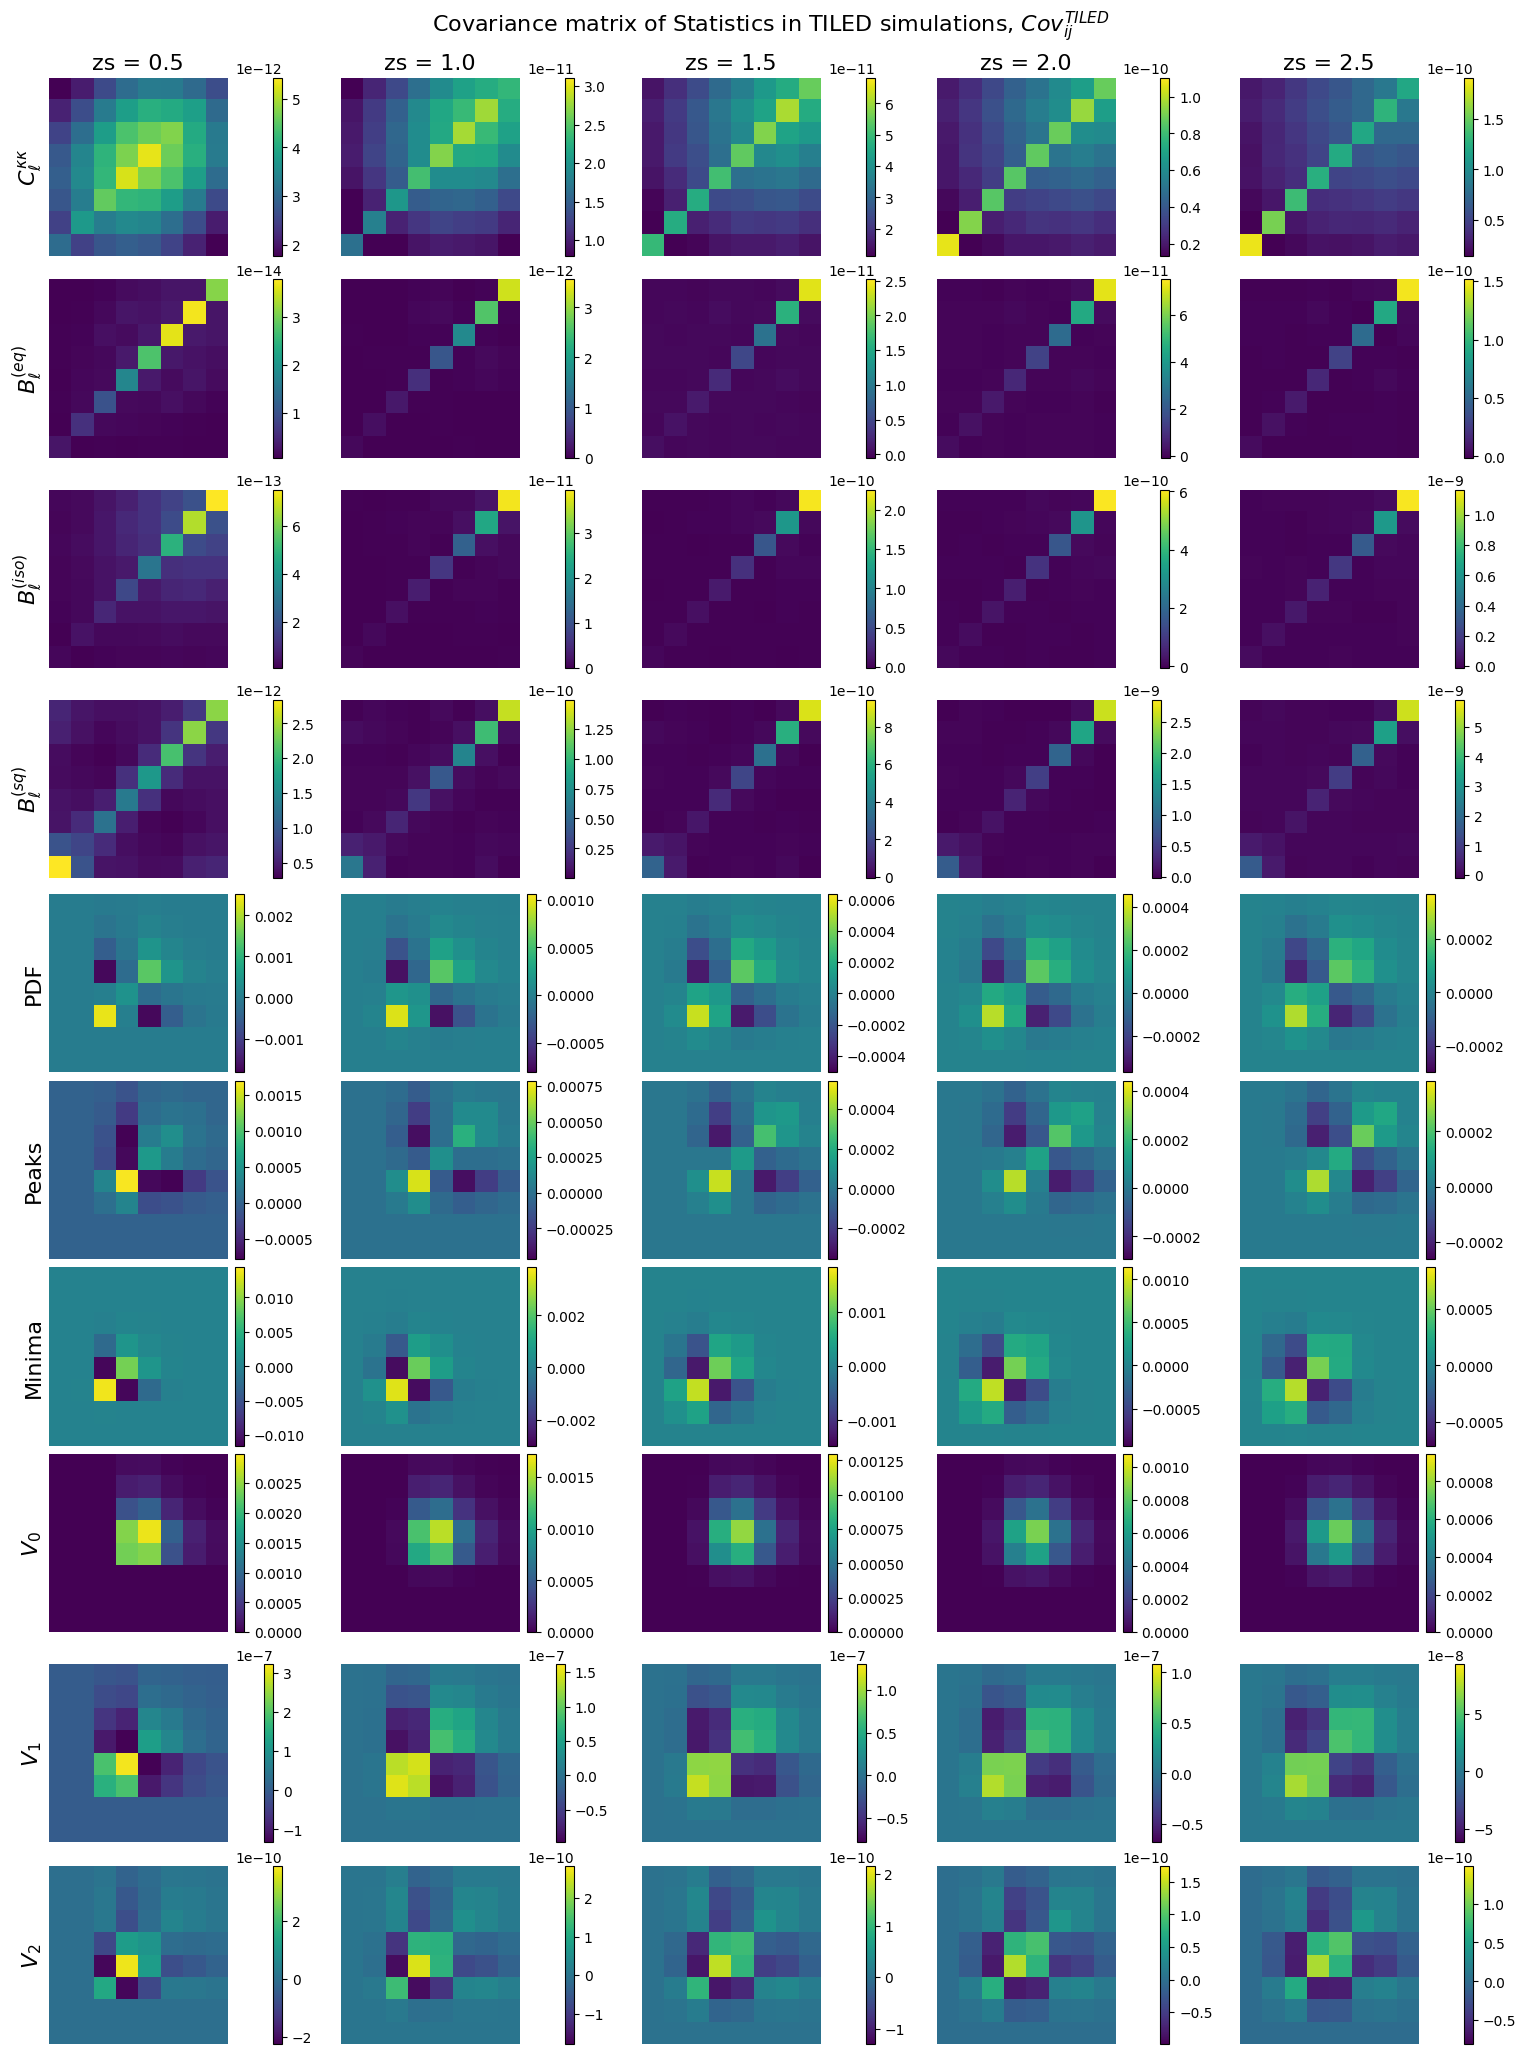
\includegraphics[width=\textwidth]{figures/results/cov_tiled.png}
    \caption[Covariance Matrices of summary statistics in TILED Simulations]{Covariance matrices of summary statistics in the TILED simulations across multiple source redshifts, using a color scale consistent with Figure~\ref{fig:cov_bigbox}.}
    \label{fig:cov_tiled}
\end{figure}

\begin{figure}[p]
    \centering
    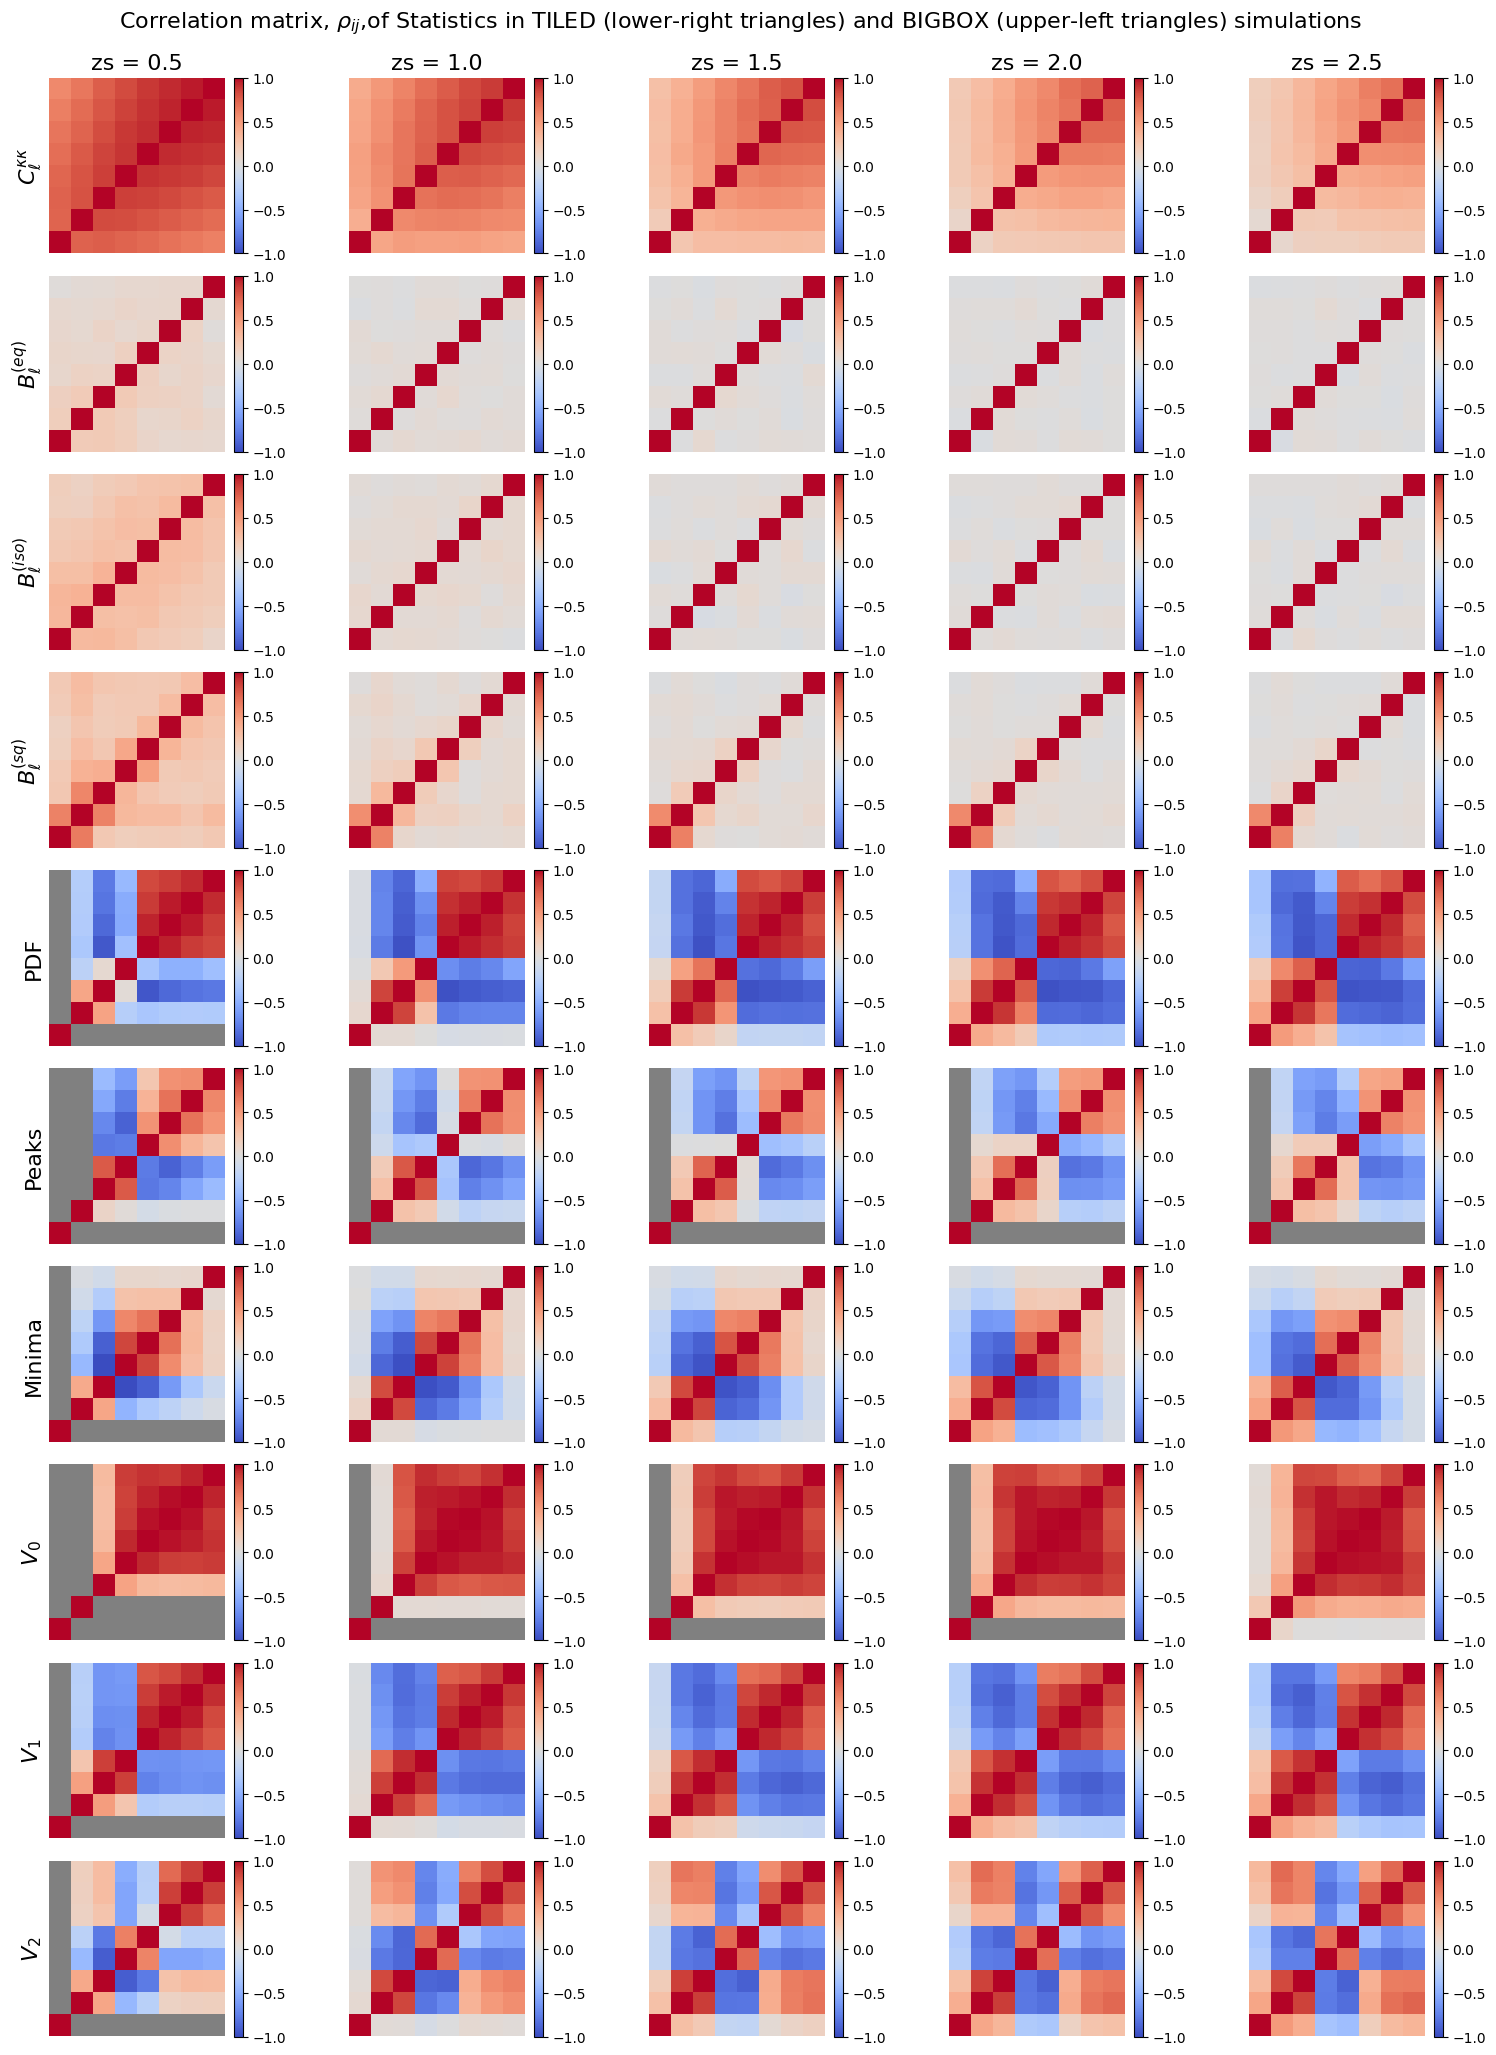
\includegraphics[width=\textwidth]{figures/results/corr_main.png}
    \caption[Correlation Matrices of summary statistics in BIGBOX and TILED Simulations]{Correlation matrices of summary statistics in the BIGBOX and TILED simulations across multiple source redshifts. The upper-left triangle contains correlation coefficients from BIGBOX simulations, and the lower-right triangle displays values from TILED simulations.}
    \label{fig:corr_main}
\end{figure}

\begin{figure}[p]
    \centering
    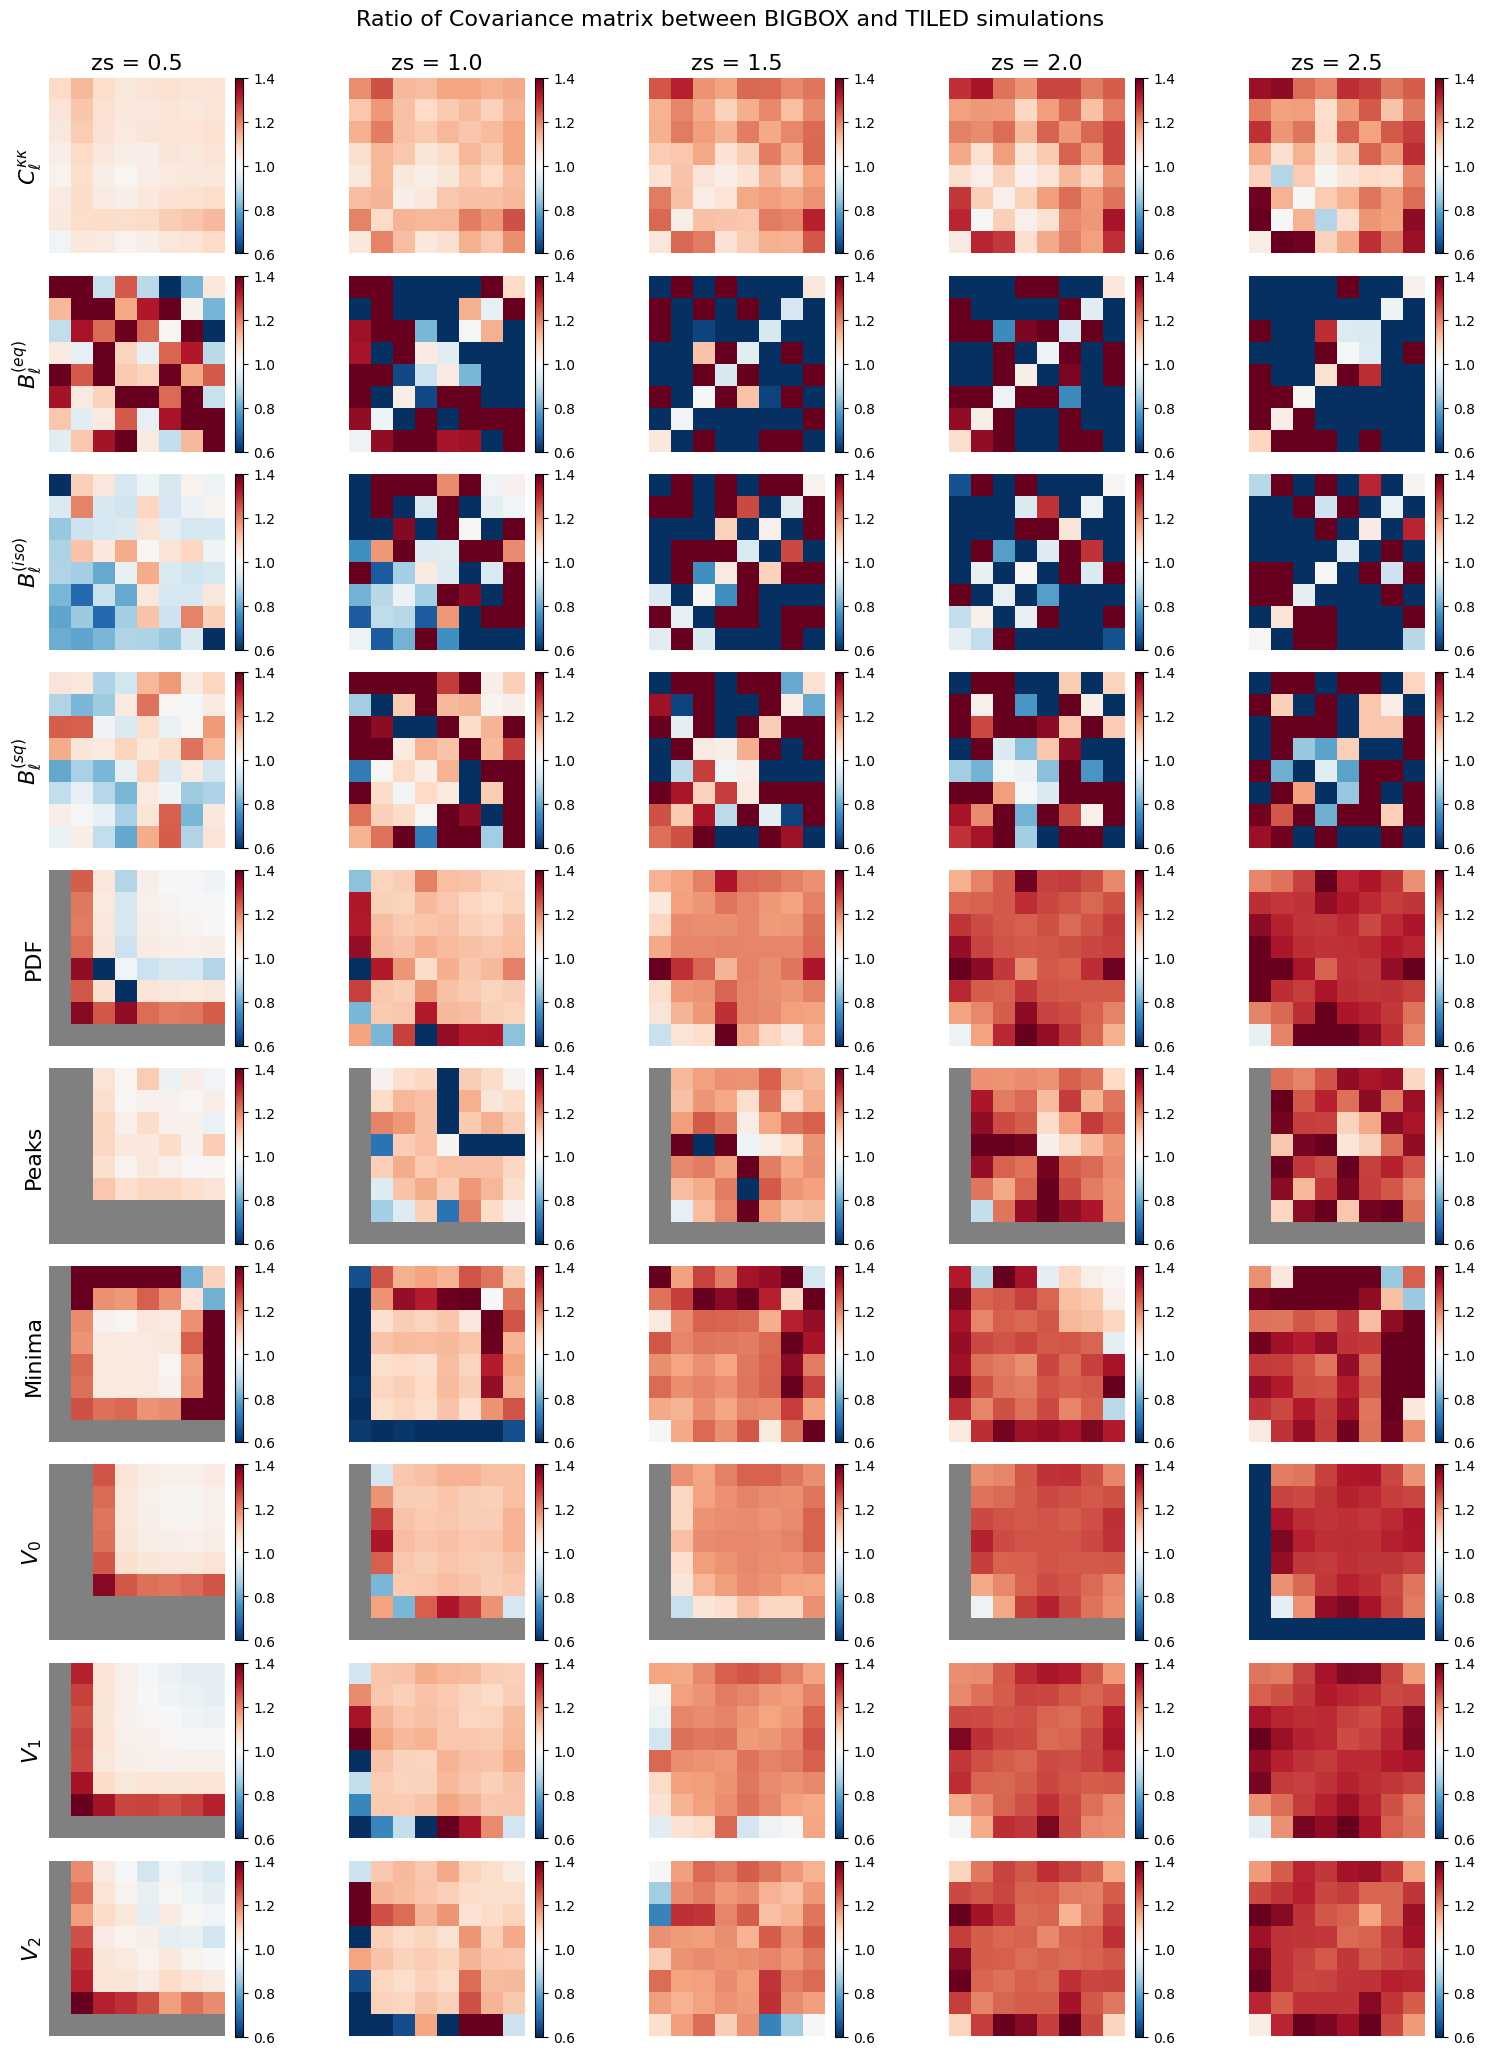
\includegraphics[width=\textwidth]{figures/results/cov_ratio.png}
    \caption[Ratios of Covariance Matrices between BIGBOX and TILED Simulations]{Ratios of covariance matrices between the BIGBOX and TILED simulations across multiple source redshifts. The ratios are consistently $10\%$ to $30\%$ higher than unity for most measured statistics, indicating the significant impact of super-sample covariance on the covariance structure.}
    \label{fig:cov_ratio_main}
\end{figure}

\begin{figure}[p]
    \centering
    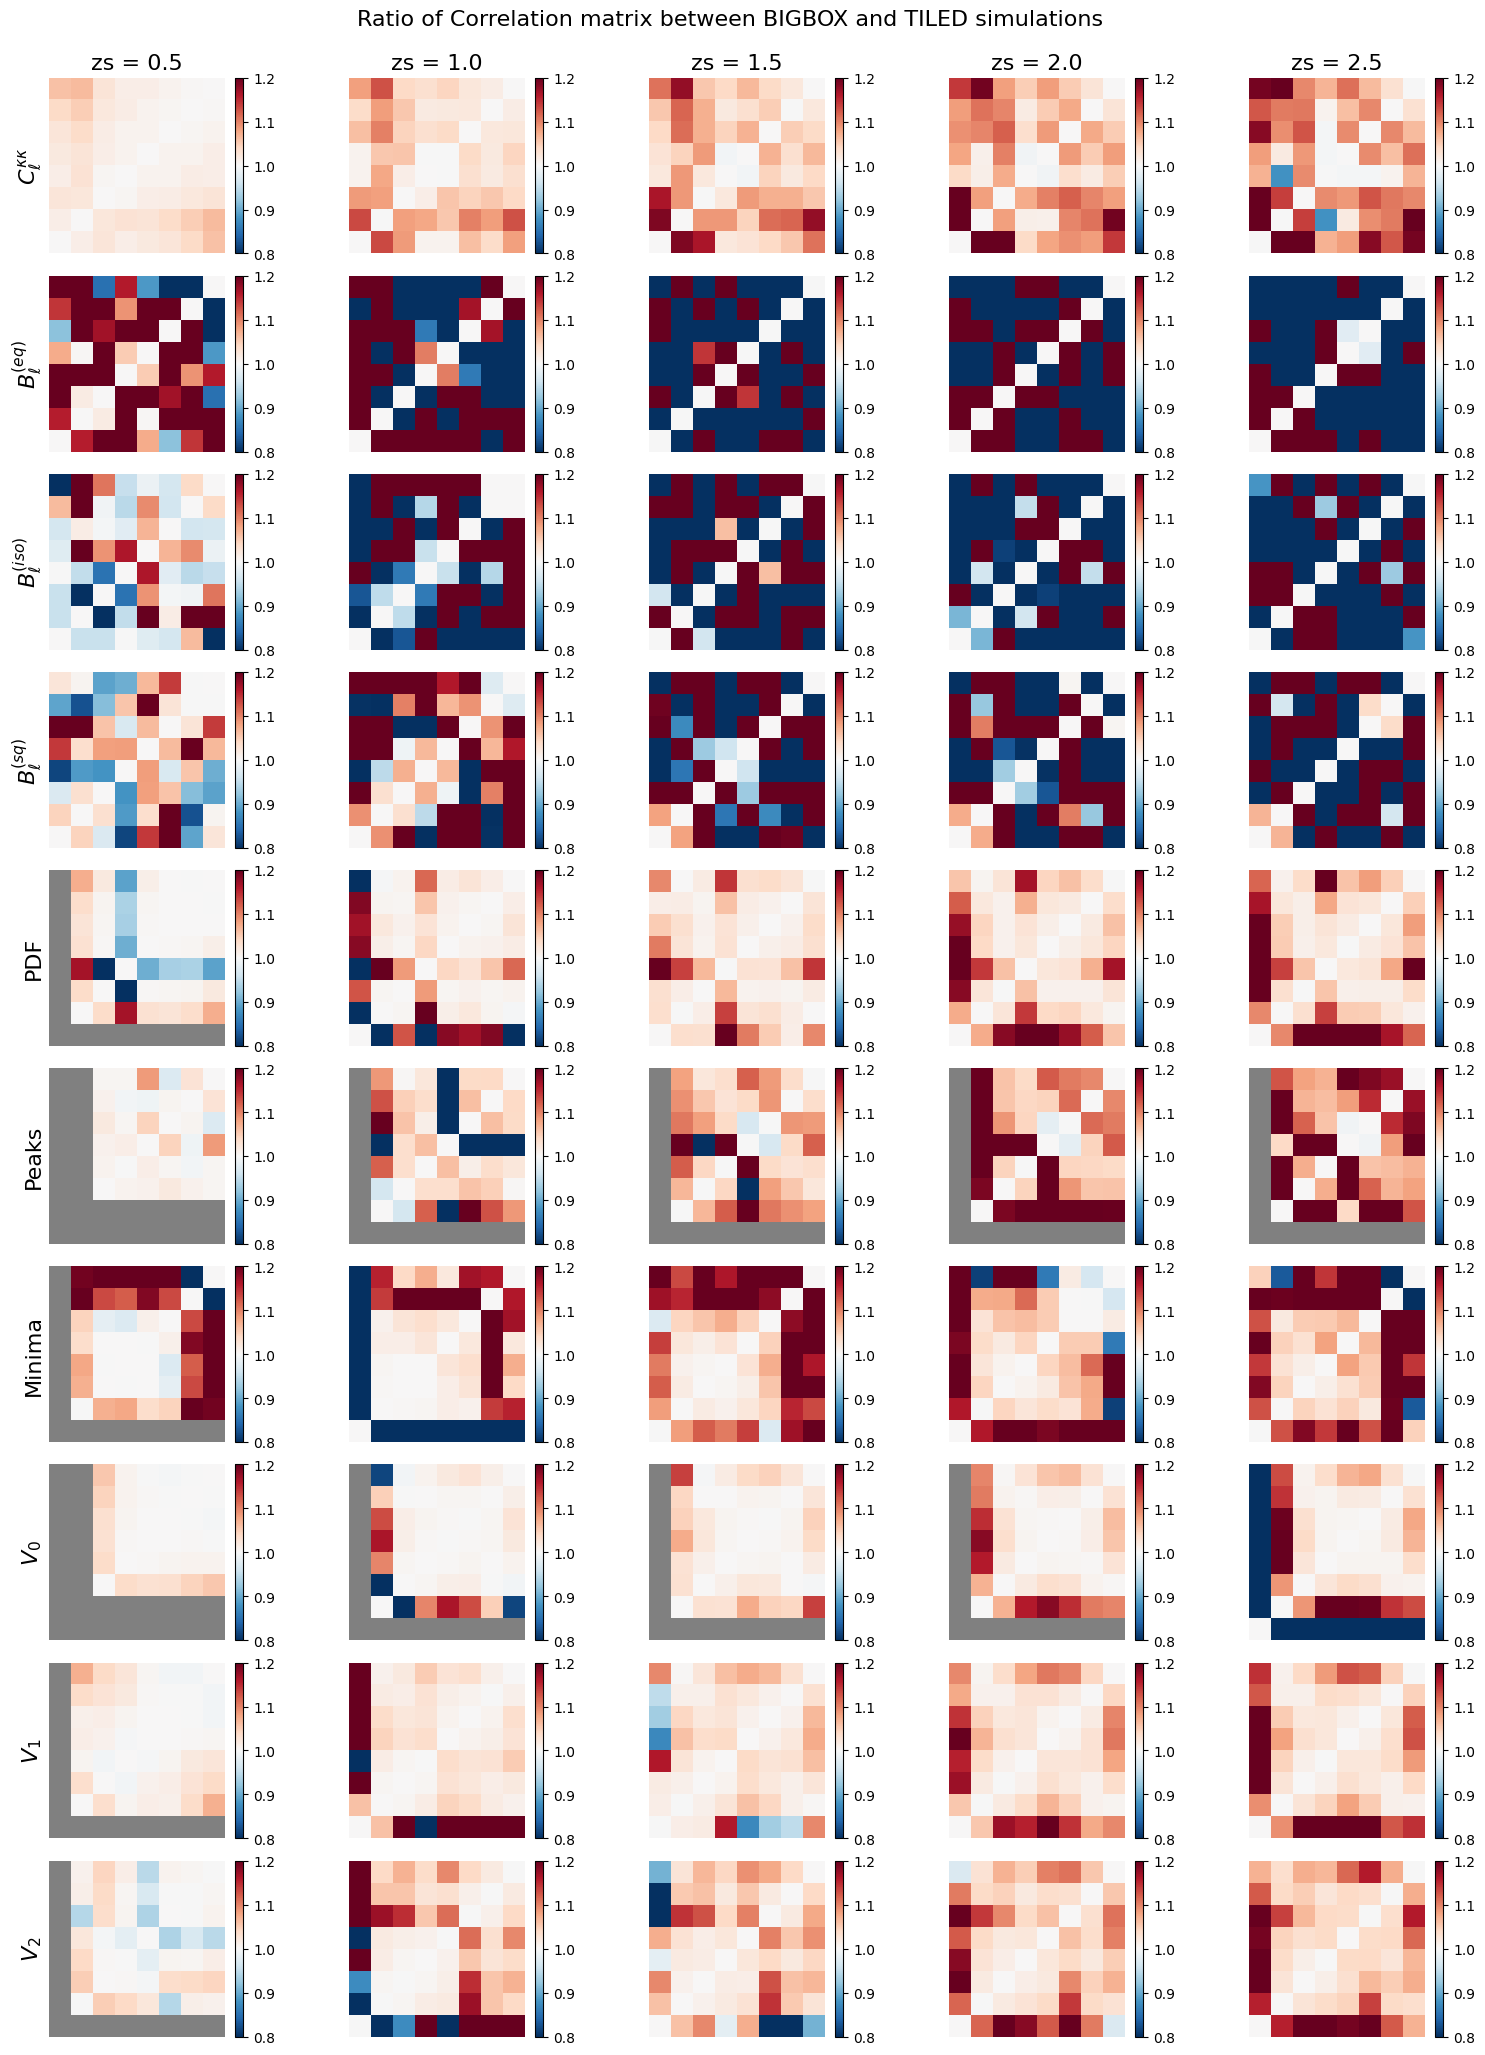
\includegraphics[width=\textwidth]{figures/results/corr_ratio.png}
    \caption[Ratios of Correlation Matrices between BIGBOX and TILED Simulations]{Ratios of correlation matrices between the BIGBOX and TILED simulations across multiple source redshifts. The ratios are generally $< 5\%$, indicating that the super-sample effect influences both diagonal and off-diagonal terms, elevating the entire covariance structure.
    }
    \label{fig:corr_ratio_main}
\end{figure}

\clearpage

\section{Effects of Noise on summary statistics}
The presence of shape noise in convergence maps can significantly affect the covariance and correlation structures of weak lensing summary statistics. To evaluate the interaction between shape noise and super-sample effects, we analyzed multiple noise levels corresponding to those expected in current and future surveys (see Table~\ref{tab:survey_comparison}). This analysis aims to quantify the extent to which the super-sample effect dominates over the contribution from shape noise. Since the bispectrums exhibit no clear trends in the noiseless case (as shown in Figures~\ref{fig:cov_ratio_main} and~\ref{fig:corr_ratio_main}), we focus our analysis on the angular power spectrum and select higher-order statistics.

Figures~\ref{fig:avg_cov_noise} and~\ref{fig:cov_noise} present the covariance matrix ratios and their averages across summary statistics for the BIGBOX and TILED simulations at various noise levels. While the angular power spectrum and peak/minima counts exhibit greater sensitivity to noise, particularly at high noise levels (e.g., DES and HSC surveys), the covariance ratios consistently exhibit an increasing trend across most statistics. This observation suggests that, in future surveys, the super-sample effect is expected to dominate over the noise contribution.

In contrast, Figures~\ref{fig:avg_corr_noise} and~\ref{fig:corr_noise} display the correlation matrix ratios and their averages across summary statistics at different noise levels. These ratios generally remain below $10\%$ for most statistics, indicating that noise has a minimal impact on the overall covariance structure. Higher values in the correlation ratios are concentrated near the boundaries of each summary statistic. These elevated ratios arise from regions where data points are sparse, rendering the measurements more susceptible to noise amplification.

\begin{figure}[p]
    \centering
    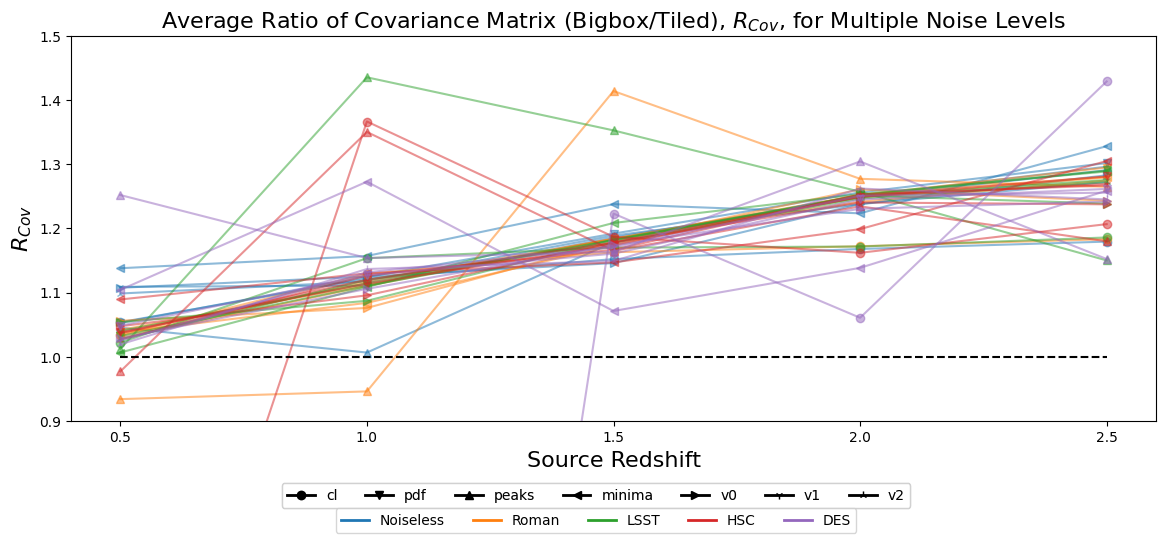
\includegraphics[width=0.95\textwidth]{figures/results/avg_cov_ratio_noise.png}
    \caption[Average BIGBOX/TILED Ratio of Covariance for Multiple Noise Levels]
    {Average ratio of covariance matrices for summary statistics between the BIGBOX and TILED simulations at different shape noise levels (see Table~\ref{tab:survey_comparison}). While the angular power spectrum and peak/minima counts are more sensitive to noise, particularly at high levels corresponding to surveys like DES and HSC, the increasing trend in covariance ratios remains consistent across most summary statistics.}
    \label{fig:avg_cov_noise}
    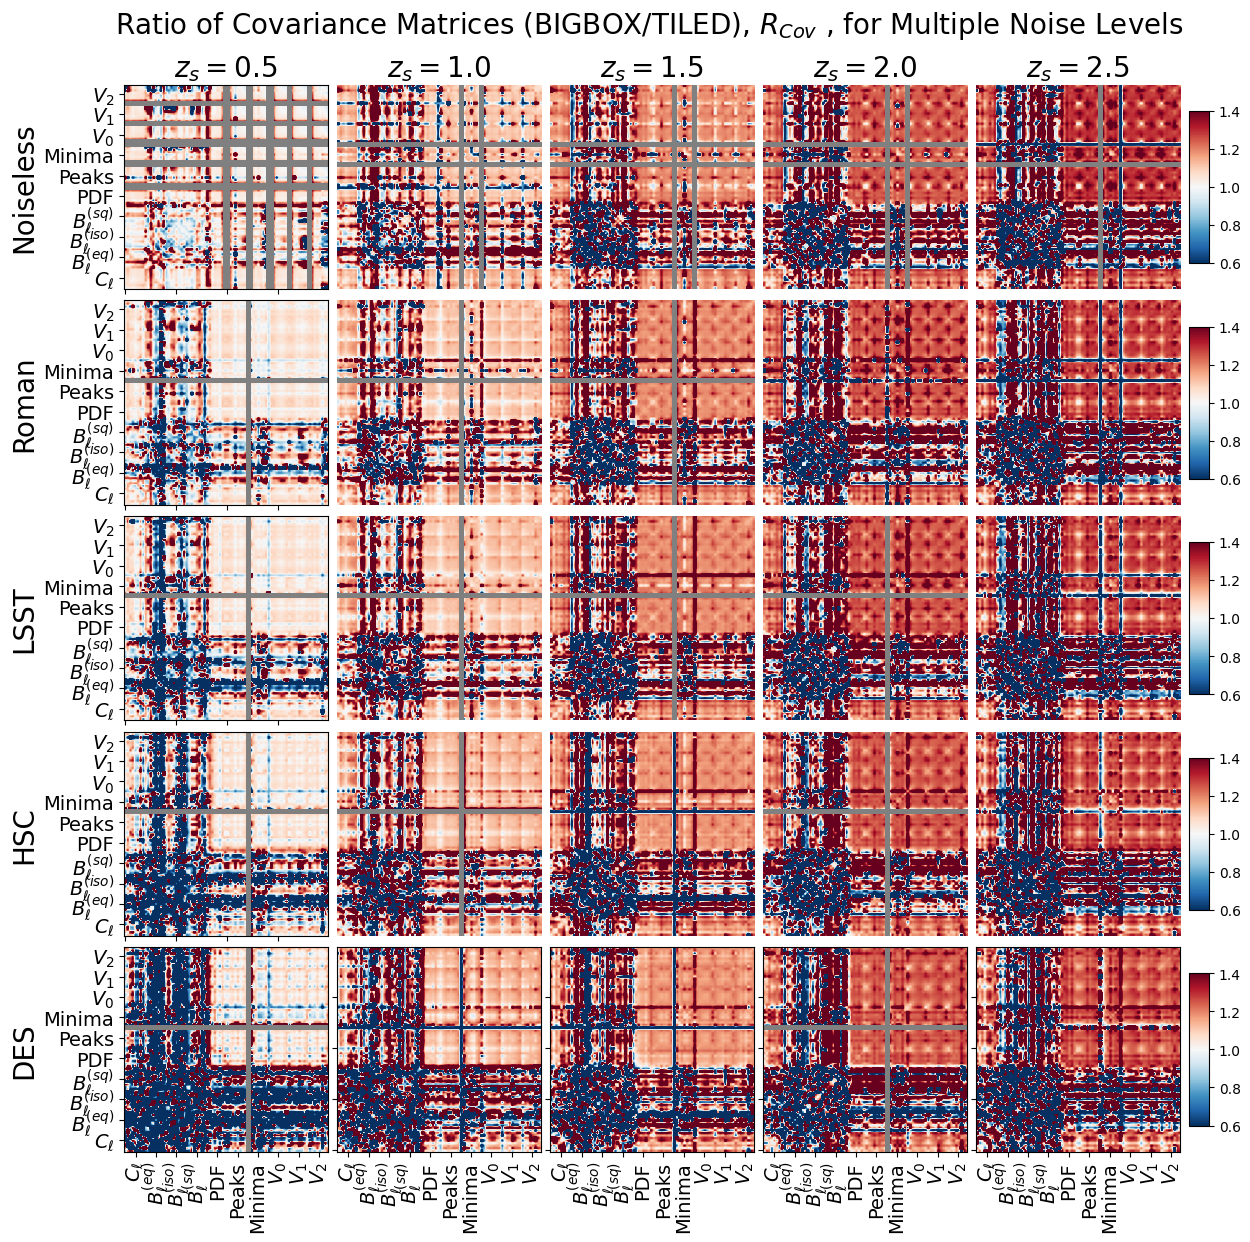
\includegraphics[width=0.95\textwidth]{figures/results/cov_noise.png}
    \caption[BIGBOX/TILED Ratio of Covariance for Multiple Noise Levels]
    {Ratio of covariance matrices for summary statistics between the BIGBOX and TILED simulations at varying shape noise levels. The covariance ratios exhibit a consistent increasing trend, highlighting the persistent influence of super-sample covariance across varying noise conditions.}
    \label{fig:cov_noise}
\end{figure}

\begin{figure}[p]
    \centering
    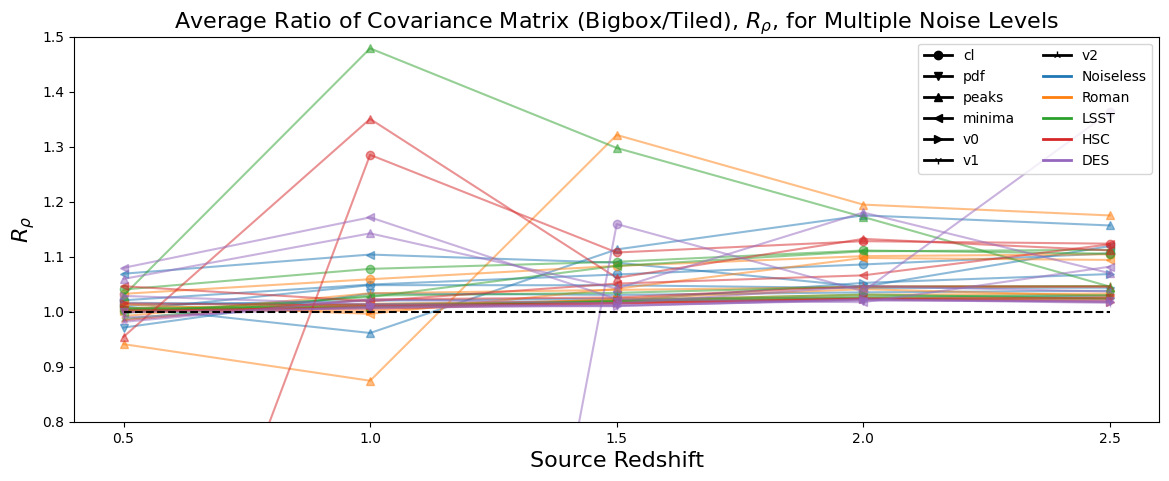
\includegraphics[width=0.95\textwidth]{figures/results/avg_corr_ratio_noise.png}
    \caption[Average BIGBOX/TILED Ratio of Correlation for Multiple Noise Levels]
    {Average ratio of correlation matrices for summary statistics between the BIGBOX and TILED simulations at varying shape noise levels (see Table~\ref{tab:survey_comparison}). While the angular power spectrum, peak counts, and minima counts exhibit greater sensitivity to noise, the correlation ratios remain below $10\%$ for most summary statistics.}
    \label{fig:avg_corr_noise}
    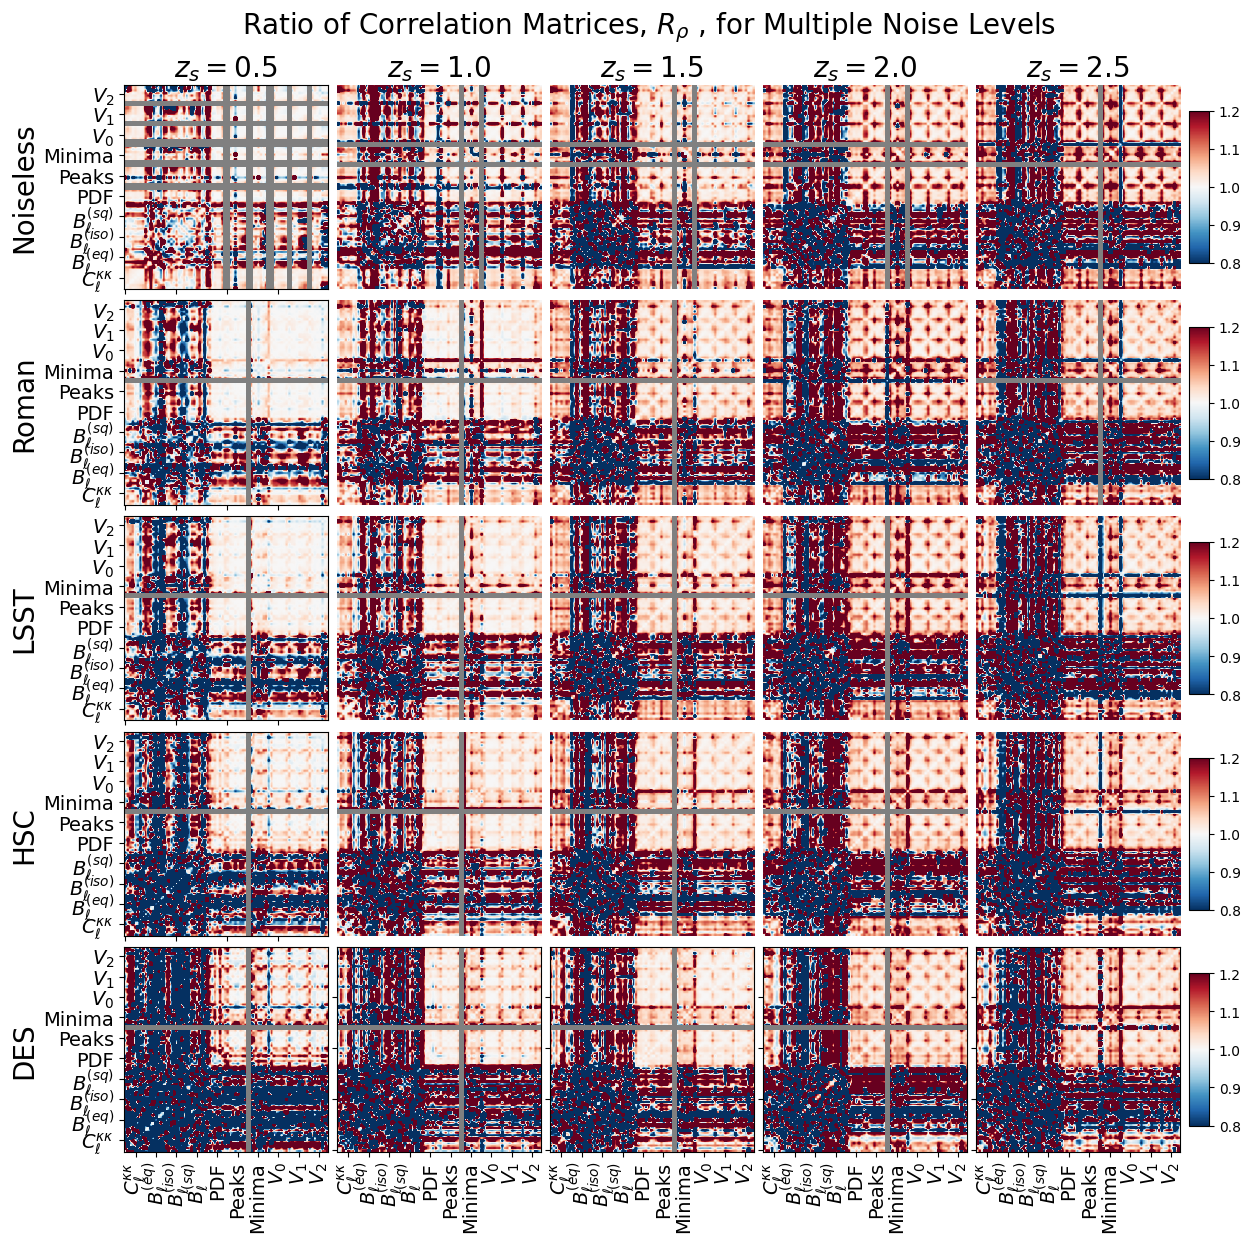
\includegraphics[width=0.95\textwidth]{figures/results/corr_noise.png}
    \caption[BIGBOX/TILED Ratio of Correlation for Multiple Noise Levels]
    {Ratio of correlation matrices for summary statistics between the BIGBOX and TILED simulations at different shape noise levels. High correlation ratios are primarily concentrated near the boundaries of summary statistics, due to sparse data points and amplified noise effects.}
    \label{fig:corr_noise}
\end{figure}

\clearpage

\section{Influence of Smoothing Scale}
We analyze the impact of varying Gaussian smoothing scales on higher-order summary statistics derived from convergence maps, with a focus on how smoothing alters their underlying structures. Increasing the smoothing scale progressively suppresses small-scale features, redistributing signal intensities across scales. Notably, smoothed convergence maps were not utilized for the calculation of the angular power spectrum and bispectrum; thus, the results are presented exclusively for other higher-order statistics.

Figures~\ref{fig:avg_cov_sl} and~\ref{fig:cov_smoothing} illustrate the changes in covariance matrix ratios and their averages as a function of the Gaussian smoothing scale. Across all smoothing scales, the average covariance ratios between the BIGBOX and TILED simulations exhibit a consistent upward trend for most summary statistics. However, notable variations occur in the peak and minima counts, particularly at larger smoothing scales. These variations are attributed to the averaging methodology, where contributions from the edges of $\nu$ bins and peak bins become increasingly significant at higher smoothing levels.

Figures~\ref{fig:avg_corr_sl} and~\ref{fig:corr_smoothing} present the ratios of correlation matrices and their averages across different Gaussian smoothing scales. The correlation ratios generally remain below $5\%$ for most summary statistics, indicating that the overall structure of the covariance matrix is robust to variations in smoothing scale. However, similar to the covariance trends, peak and minima counts exhibit elevated correlation ratios, particularly at larger smoothing scales.

In summary, these findings suggest that while Gaussian smoothing scales can influence individual summary statistics, the overall structural integrity of the covariance and correlation matrices remains largely unaffected by changes in smoothing scale.

\begin{figure}[p]
    \centering
    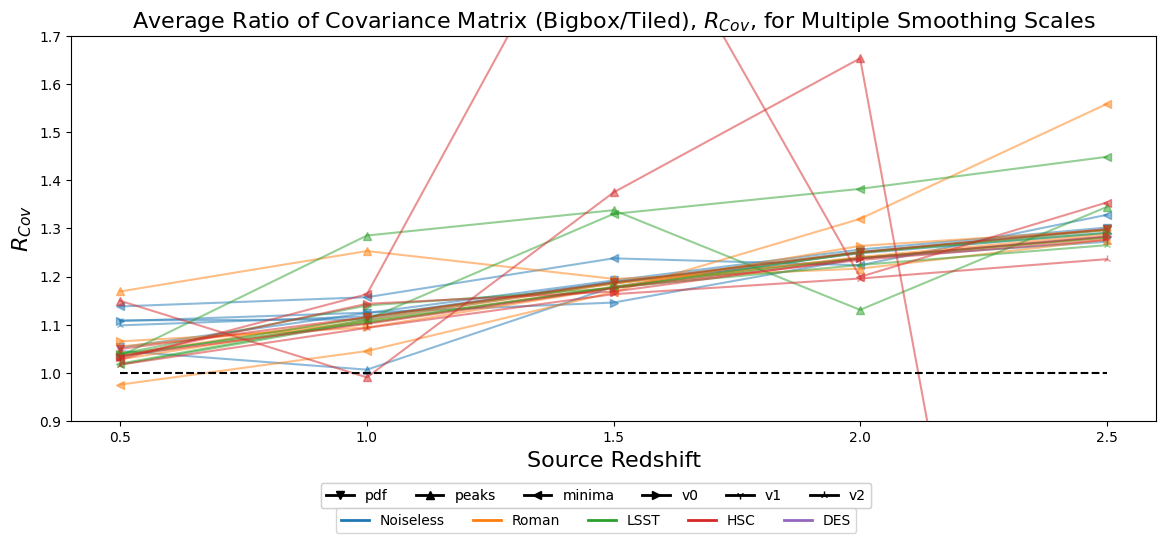
\includegraphics[width=\textwidth]{figures/results/avg_cov_ratio_sl.png}
    \caption[Average BIGBOX/TILED Ratio of Covariance for Multiple Smoothing Scales]
    {Average ratio of covariance matrices for various summary statistics between the BIGBOX and TILED simulations at differing Gaussian smoothing scales, illustrating the effect of smoothing on covariance ratios. The overall increasing trend persists across all smoothing scales, with pronounced variations in peak and minima counts becoming more evident at larger smoothing scales, due to the increased significance of edge contributions in $\nu$ bins.}
    \label{fig:avg_cov_sl}
    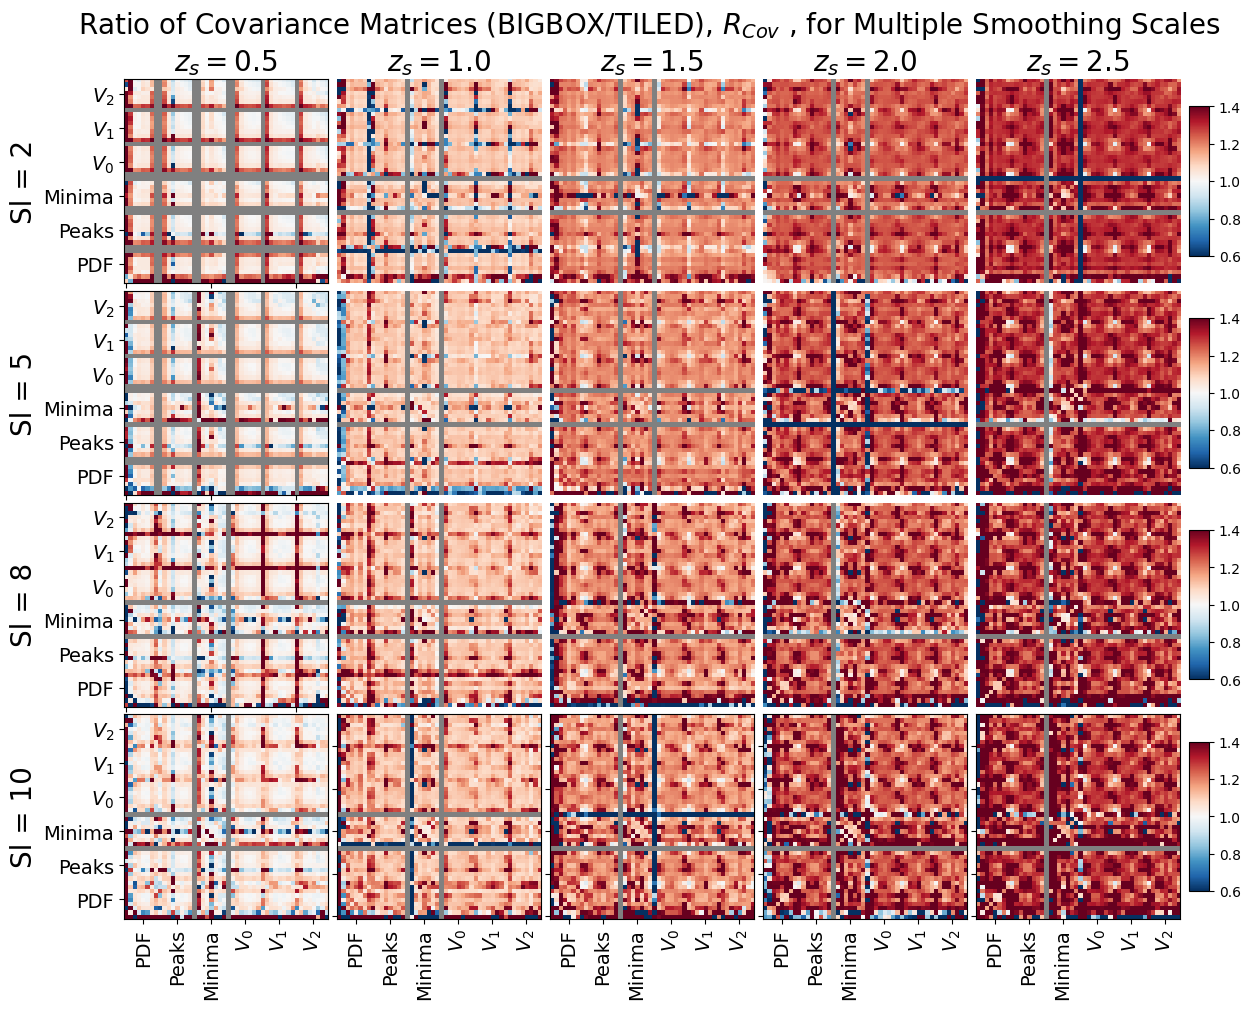
\includegraphics[width=\textwidth]{figures/results/cov_smoothing.png}
    \caption[BIGBOX/TILED Ratio of Covariance for Multiple Smoothing Scales]
    {Ratio of covariance matrices for various summary statistics between the BIGBOX and TILED simulations across different Gaussian smoothing scales, highlighting the consistent trends in covariance ratios regardless of the applied smoothing scale.}
    \label{fig:cov_smoothing}
\end{figure}

\begin{figure}[p]
    \centering
    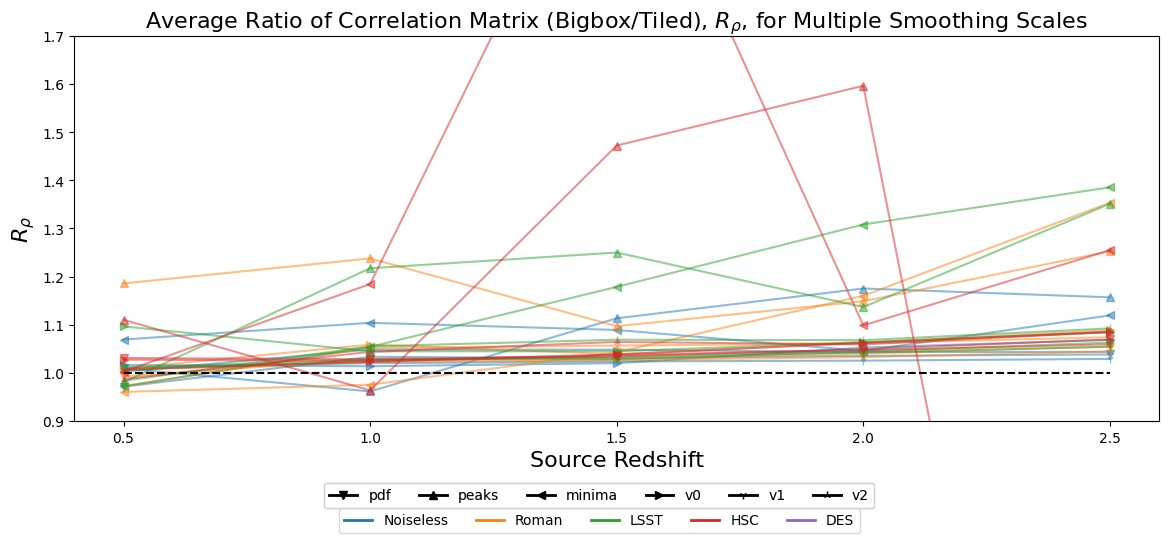
\includegraphics[width=\textwidth]{figures/results/avg_corr_ratio_sl.png}
    \caption[Average BIGBOX/TILED Ratio of Correlation for Multiple Smoothing Scales]
    {Average ratio of correlation matrices for various summary statistics between the BIGBOX and TILED simulations at different Gaussian smoothing scales. Correlation ratios predominantly remain below $5\%$ for most summary statistics, highlighting the limited influence of smoothing on the overall correlation structure. Peak and minima counts, however, exhibit larger variations at higher smoothing scales, driven by edge effects in $\nu$ bins.}
    \label{fig:avg_corr_sl}
    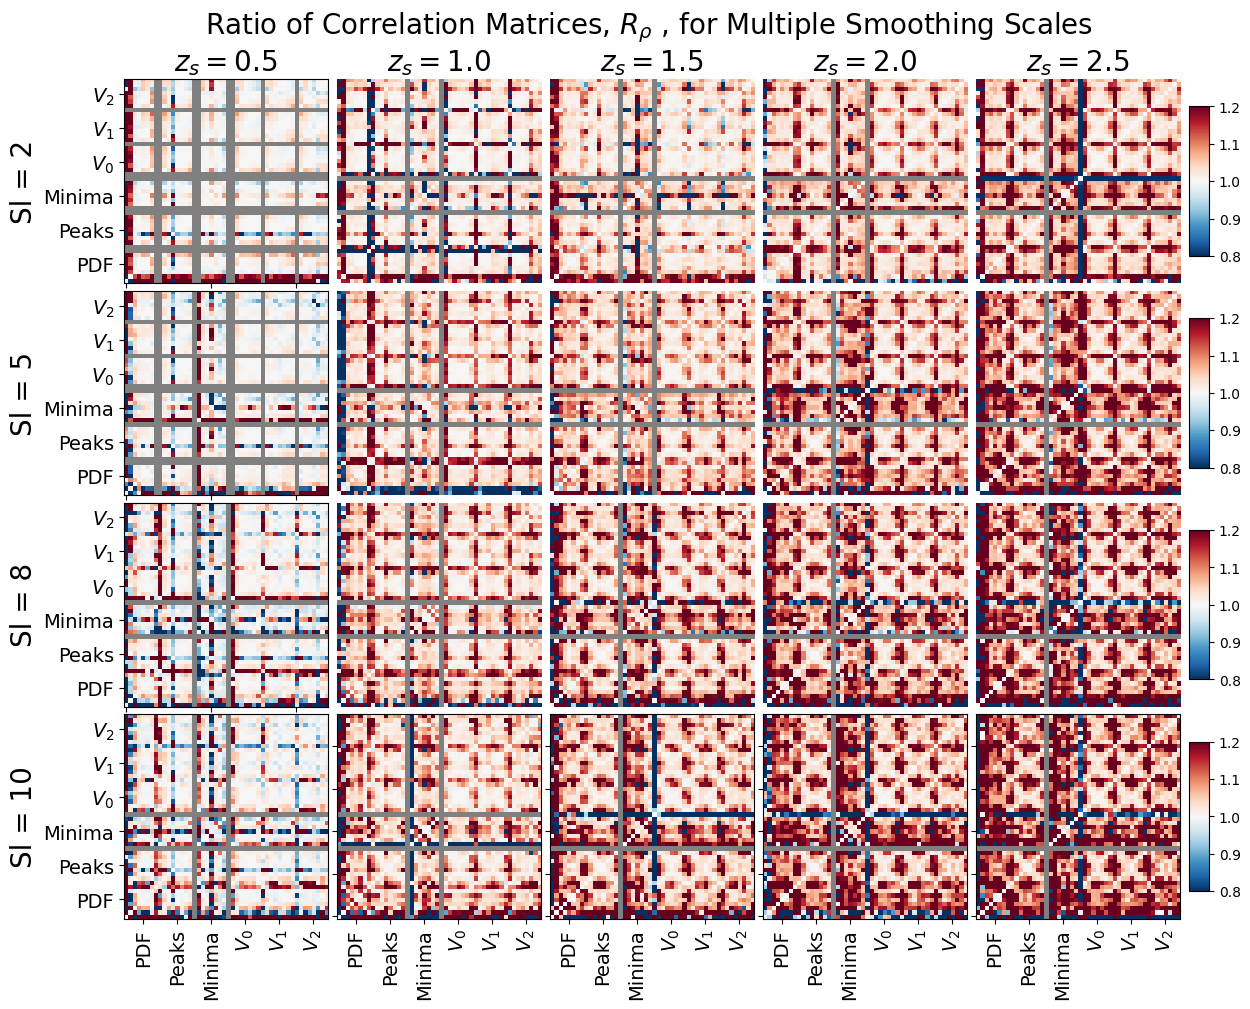
\includegraphics[width=\textwidth]{figures/results/corr_smoothing.png}
    \caption[BIGBOX/TILED Ratio of Correlation for Multiple Smoothing Scales]
    {Ratio of correlation matrices for various summary statistics between the BIGBOX and TILED simulations across different Gaussian smoothing scales. Apart from near the boundaries of $\nu$ bins, the correlation ratios remain consistently modest across all smoothing scales.} 
    \label{fig:corr_smoothing}
\end{figure}

\clearpage

\section{Systematic Effects: Box Replication Artifact} \label{sec:boxreplication}
In weak lensing simulations, extending the simulated volume often requires replicating finite simulation boxes to create a larger effective volume. This box replication process can inadvertently introduce artificial correlations in the data, particularly near the boundaries or along preferred replication directions. These artifacts can potentially compromise the reliability of higher-order summary statistics. To systematically investigate this issue, we categorize simulation regions into two groups: regions where artifacts are significant, termed \textbf{Replication-Influenced Patches (RIP)}, and regions minimally affected by artifacts, termed \textbf{Replication-Minimal Patches (RMP)}.
The criteria for categorizing patches are as follows:
\begin{itemize} 
    \item Replication-Influenced Patches (RIP):
    \begin{itemize}
        \item Patches near the equator: $ \left| \theta_i - \frac{\pi}{2} \right| \leq R_{\text{patch}} $ 
        \item Patches near the edges of octants: $ \left| \phi_i - \frac{k\pi}{2} \right| \leq R_{\text{patch}} $ for $k = 0, 1, 2, 3$
    \end{itemize}
    \item Replication-Minimal Patches (RMP):
    \begin{itemize}
        \item All other patches not meeting the above criteria.
    \end{itemize}
\end{itemize}
where $(\theta_i, \phi_i)$ denote the center of patch $i$, and $R_{\text{patch}} = 5\sqrt{2}\, \mathrm{\deg}$ is the half-diagonal of the patch.

Our analysis indicates that patches containing the point $(\theta_i, \phi_i) = (\pi/2, 0)$ exhibit significant deviations in both the mean and variance of summary statistics compared to other RIPs. To prevent these outliers from skewing our results, we exclude this specific point from subsequent analyses.

After these adjustments, we obtained $70$ RMP per realization, and $1400$ RMP for the TILED simulations and $770$ RMP for the BIGBOX simulations across all realizations.

Figure~\ref{fig:boxreplication_main} illustrates the ratios of mean and variance for various summary statistics between RIPs and RMPs. The analysis reveals that the mean angular power spectra in RIPs are systematically underestimated by approximately $0.5\%$. Additionally, the $\nu$-binned statistics exhibit elevated mean values in low $\nu$ bins and reduced values in high $\nu$ bins. This pattern suggests that box replication accentuates both overdense and underdense regions, leading to more extreme convergence values. In the TILED simulations, the limited resolution in underdense regions shifts the $\nu$-binned statistics toward lower $\nu$ bins. Conversely, the variance ratios approach unity, indicating that the box replication effect amplifies variance to levels comparable to those observed in the BIGBOX simulations. Notably, the dependence on source redshift is effectively nullified in RIPs, implying that box replication conceals the super-sample variance.

\begin{figure}[p] 
    \centering 
    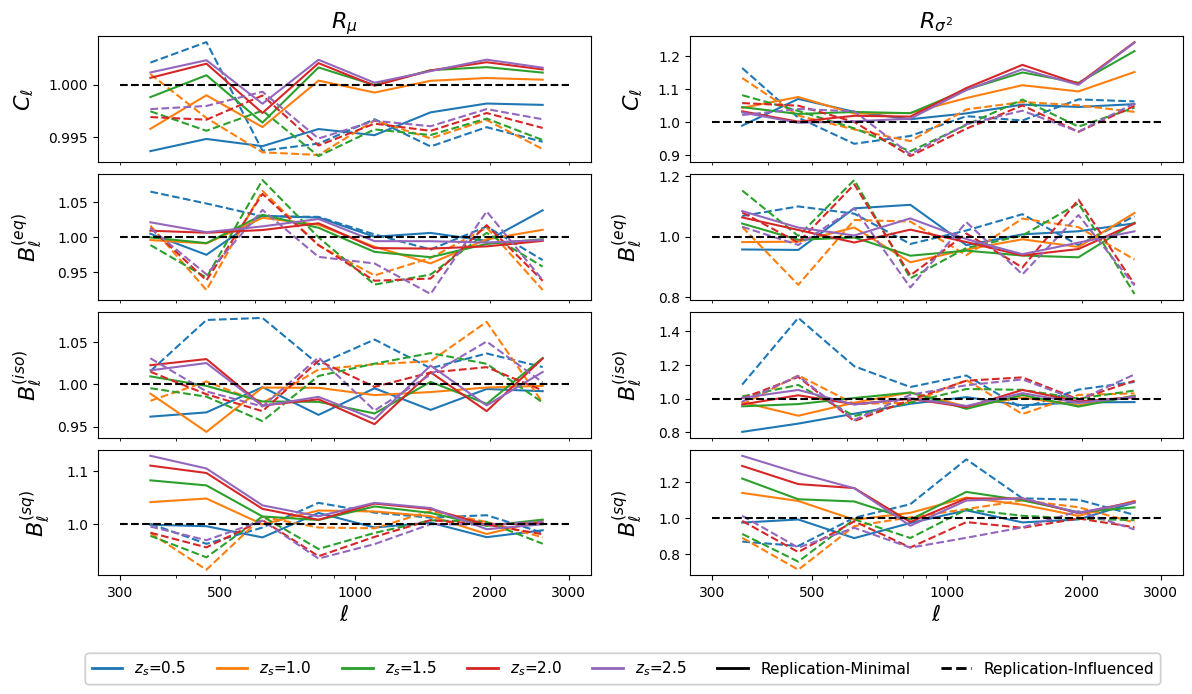
\includegraphics[width=\textwidth]{figures/results/BR_ratio_ell.png} 
    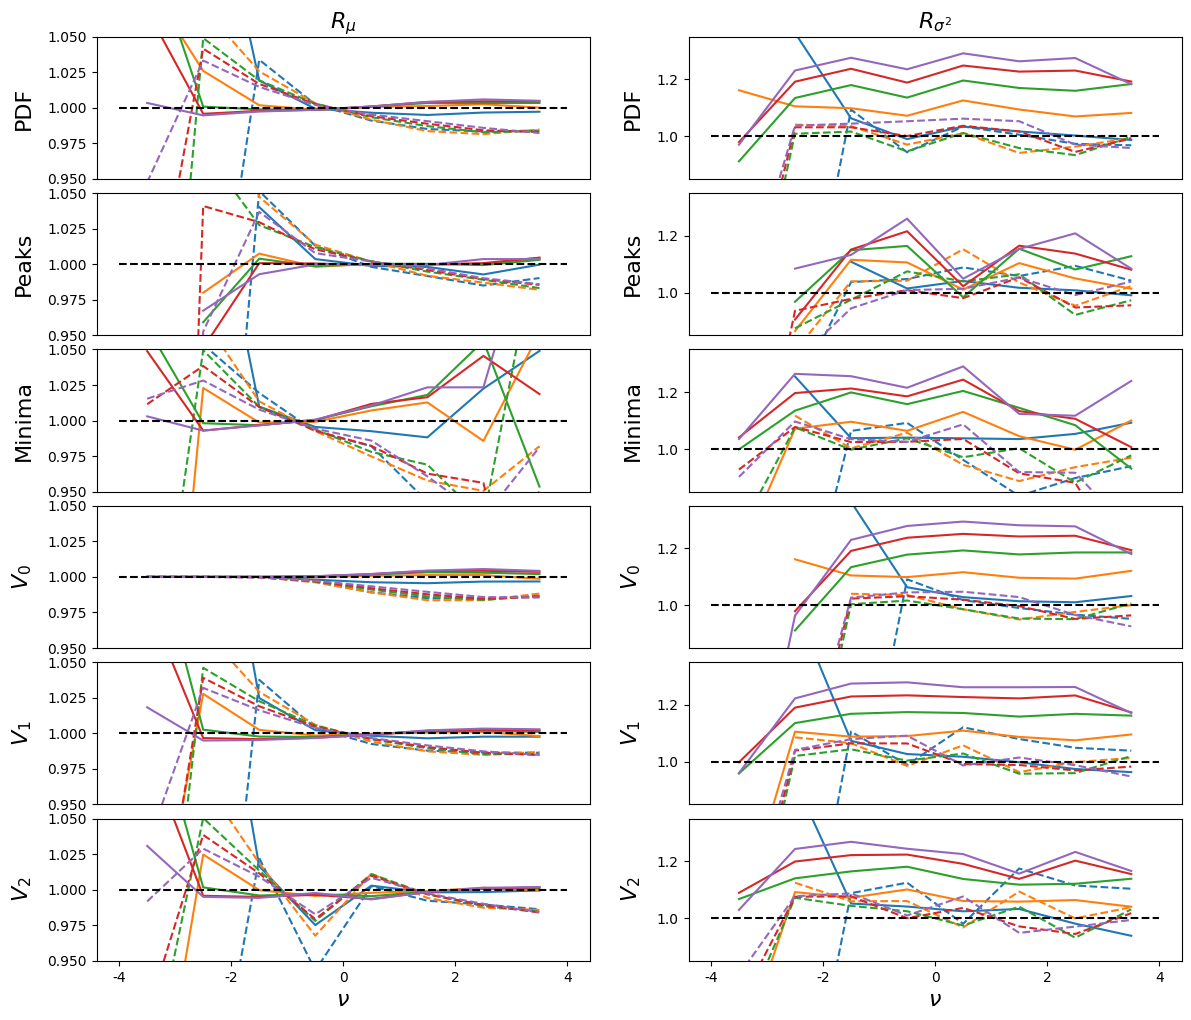
\includegraphics[width=\textwidth]{figures/results/BR_ratio_nu.png} 
    \caption[BIGBOX/TILED Ratios of the mean and variance of summary statistics for the RIPs and the RMPs]{Ratios of the mean and variance of summary statistics between Replication-Influenced Patches (RIP) and Replication-Minimal Patches (RMP). The $\nu$-binned statistics exhibit elevated mean values in low $\nu$ bins and reduced mean values in high $\nu$ bins. Variance ratios are generally close to unity, indicating that box replication amplifies variance to levels comparable to those in BIGBOX simulations.} \label{fig:boxreplication_main} 
\end{figure}

Figures~\ref{fig:boxreplication_cov_RIP} and~\ref{fig:boxreplication_corr_RIP} display the ratios of covariance and correlation matrices between TILED and BIGBOX simulations for RIPs. Additionally, Figures~\ref{fig:boxreplication_avg_cov} and~\ref{fig:boxreplication_avg_corr} present the average ratios for both RIPs and RMPs. The main observations are that RIPs consistently exhibit lower covariance ratios compared to RMPs. Similarly, the correlation ratios for RIPs are generally lower than those for RMPs, except at $z_s=0.5$, where the super-sample effect is present in both TILED and BIGBOX simulations. Furthermore, distinct covariance structures, such as those for $C_\ell$ and $V_0$, emerge due to box replication artifacts. Structural transitions observed in previous analyses occur at higher redshifts ($z_s=2.0\sim2.5$) in RIPs, aligning with RMPs as higher redshift regions become dominated by RMPs.

\begin{figure}[ht]
    \centering
    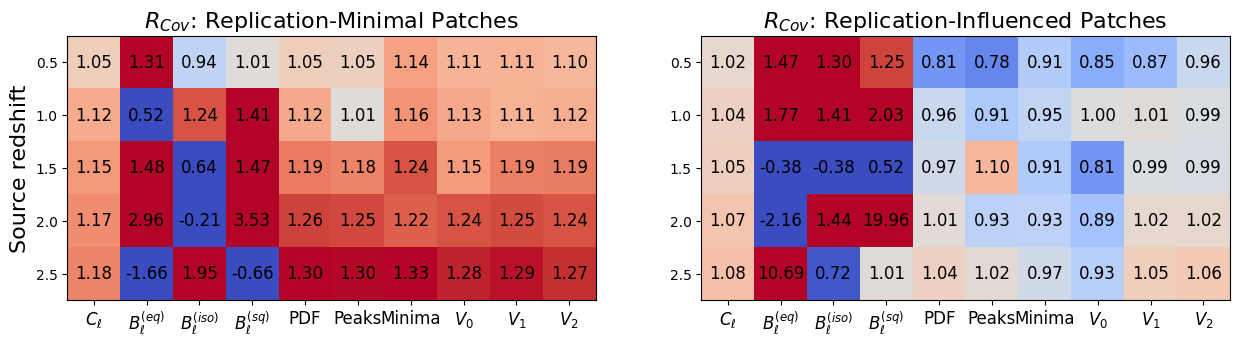
\includegraphics[width=\textwidth]{figures/results/BR_avg_cov_ratio.png}
    \caption[Average BIGBOX / TILED ratios of covariance matrices for the RIPs and the RMPs]{Average BIGBOX/TILED ratios of covariance matrices for Replication-Influenced Patches (RIP) and Replication-Minimal Patches (RMP). The ratios for RIPs (right panel) are consistently lower than those for RMPs (left panel), indicating that box replication artifacts reduce covariance ratios in replication-influenced regions.}
    \label{fig:boxreplication_avg_cov}
\end{figure}

\begin{figure}[ht]
    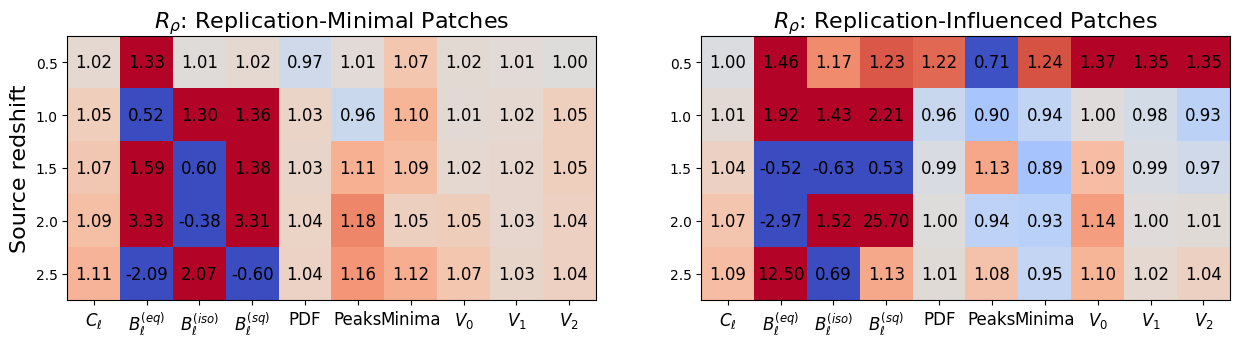
\includegraphics[width=\textwidth]{figures/results/BR_avg_corr_ratio.png}
    \caption[Average BIGBOX / TILED ratios of correlation matrices for the RIPs and the RMPs]{Average BIGBOX/TILED ratios of correlation matrices for Replication-Influenced Patches (RIP) and Replication-Minimal Patches (RMP). The ratios for RIPs (right panel) are consistently lower than those for RMPs (left panel), except at $z_s = 0.5$, where super-sample effects impact both TILED and BIGBOX simulations similarly.}
    \label{fig:boxreplication_avg_corr}
\end{figure}

\begin{figure}[p]
    \centering
    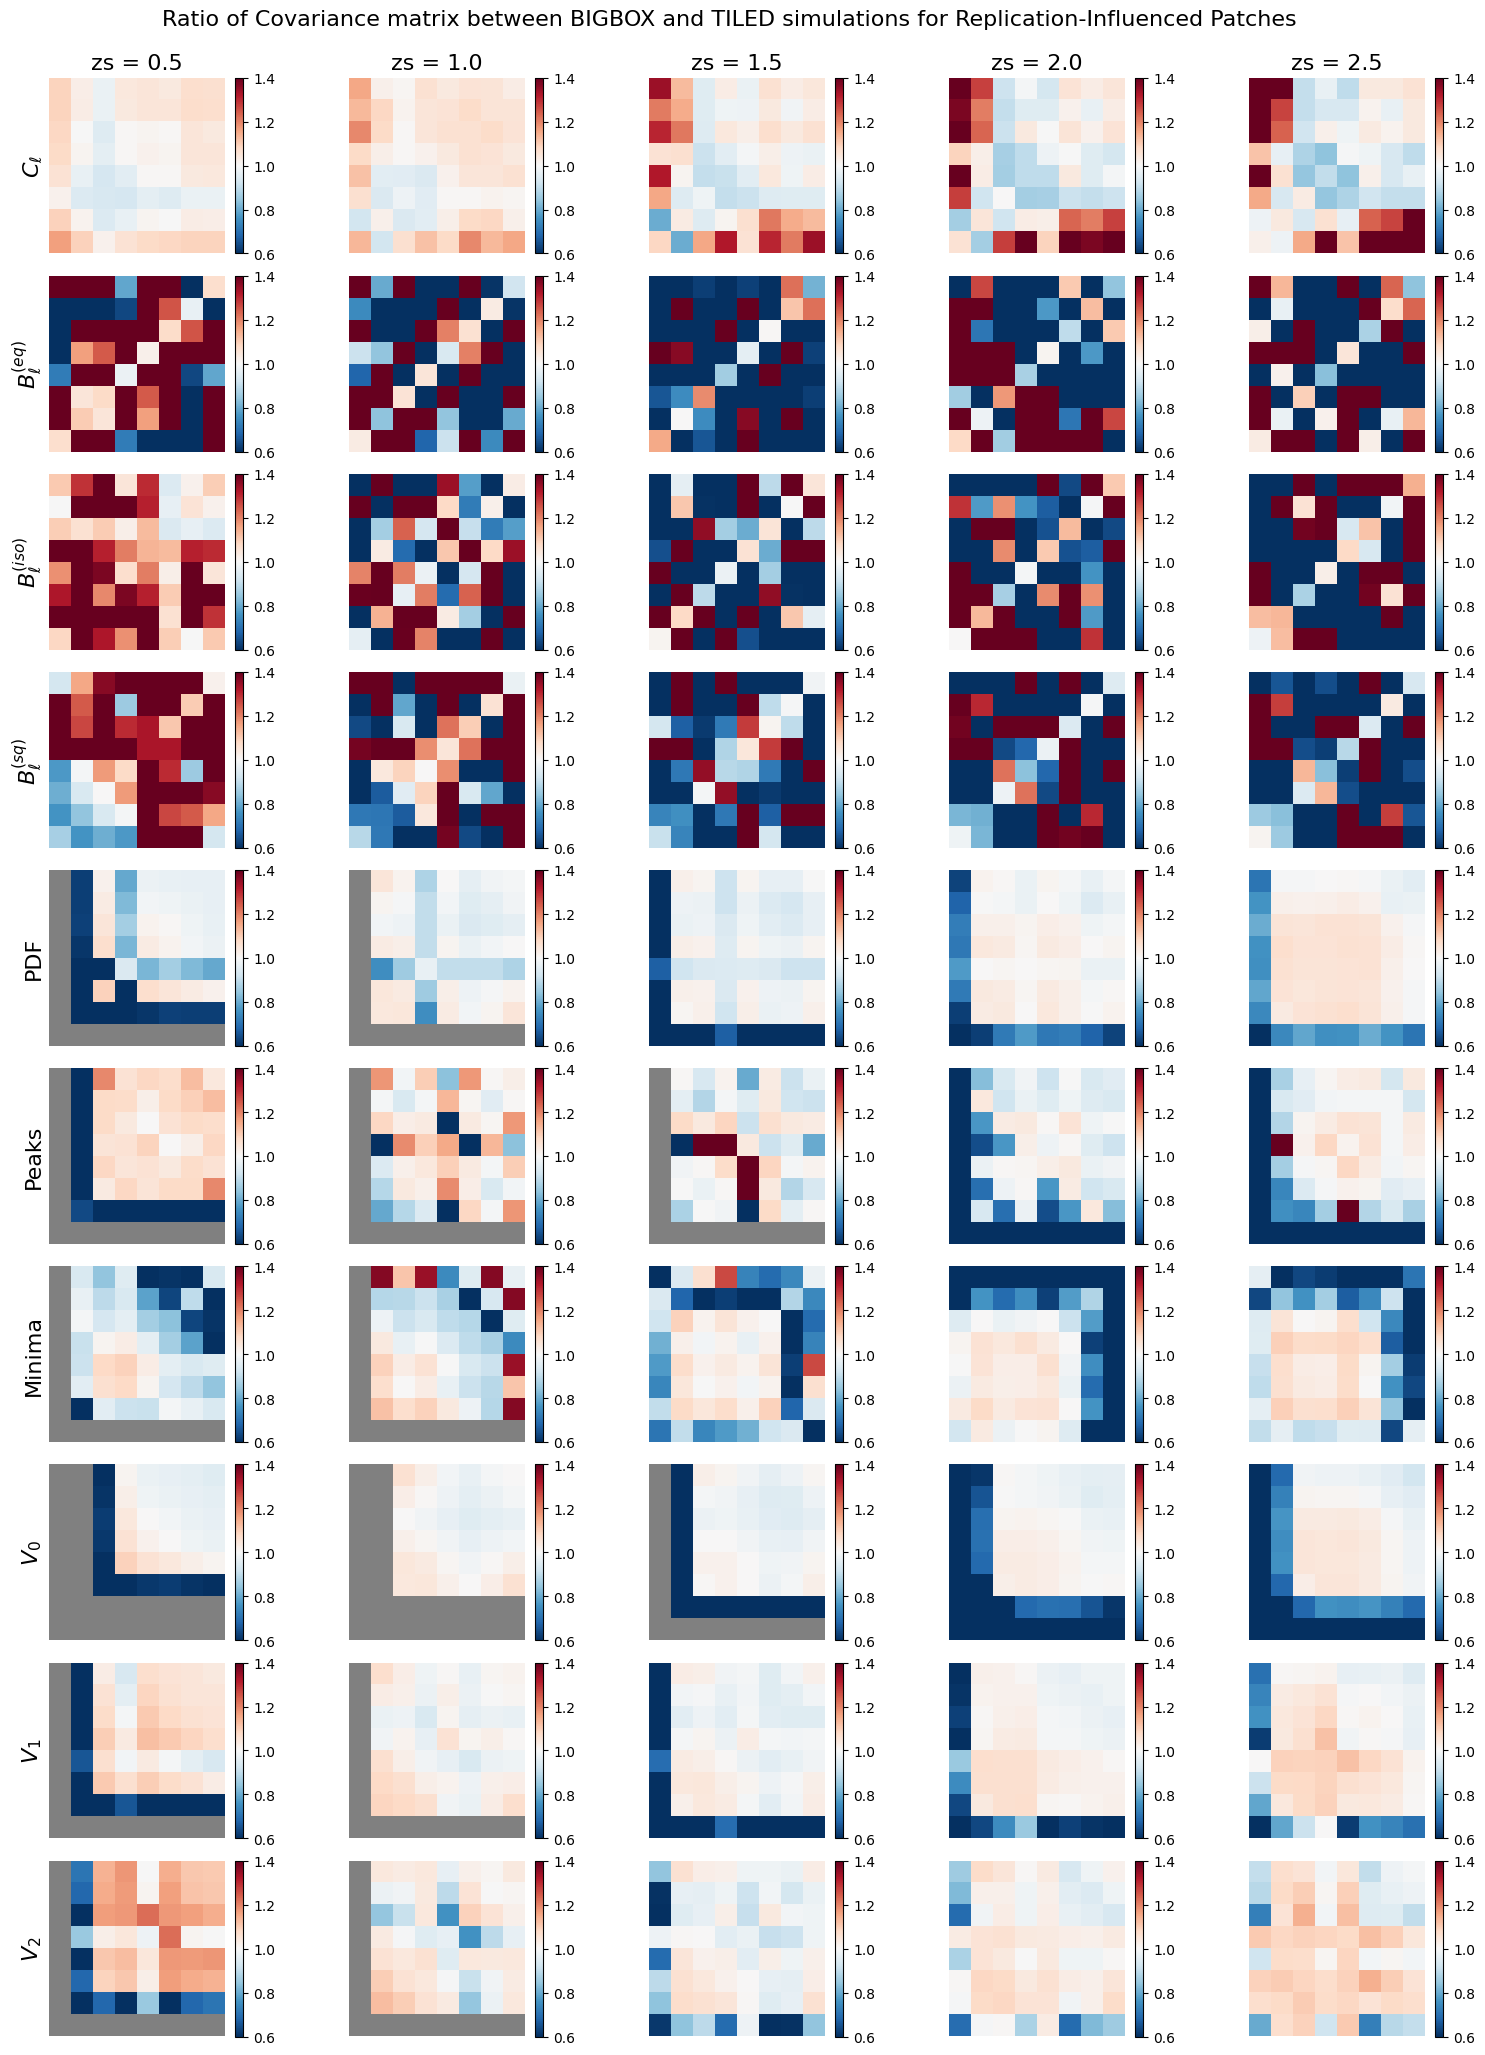
\includegraphics[width=\textwidth]{figures/results/cov_ratio_RIP.png}
    \caption[Covariance Ratios for RIP]{BIGBOX/TILED ratios of covariance matrices specifically for Replication-Influenced Patches (RIP). Compared to Figure~\ref{fig:corr_ratio_main}, RIP ratios are consistently lower than those for RMPs. Covariance structures unique to RIPs, such as $C_\ell$ and $V_0$, indicate that box replication artifacts can generate distinct covariance structures.}
    \label{fig:boxreplication_cov_RIP}
\end{figure}

\begin{figure}[p]
    \centering
    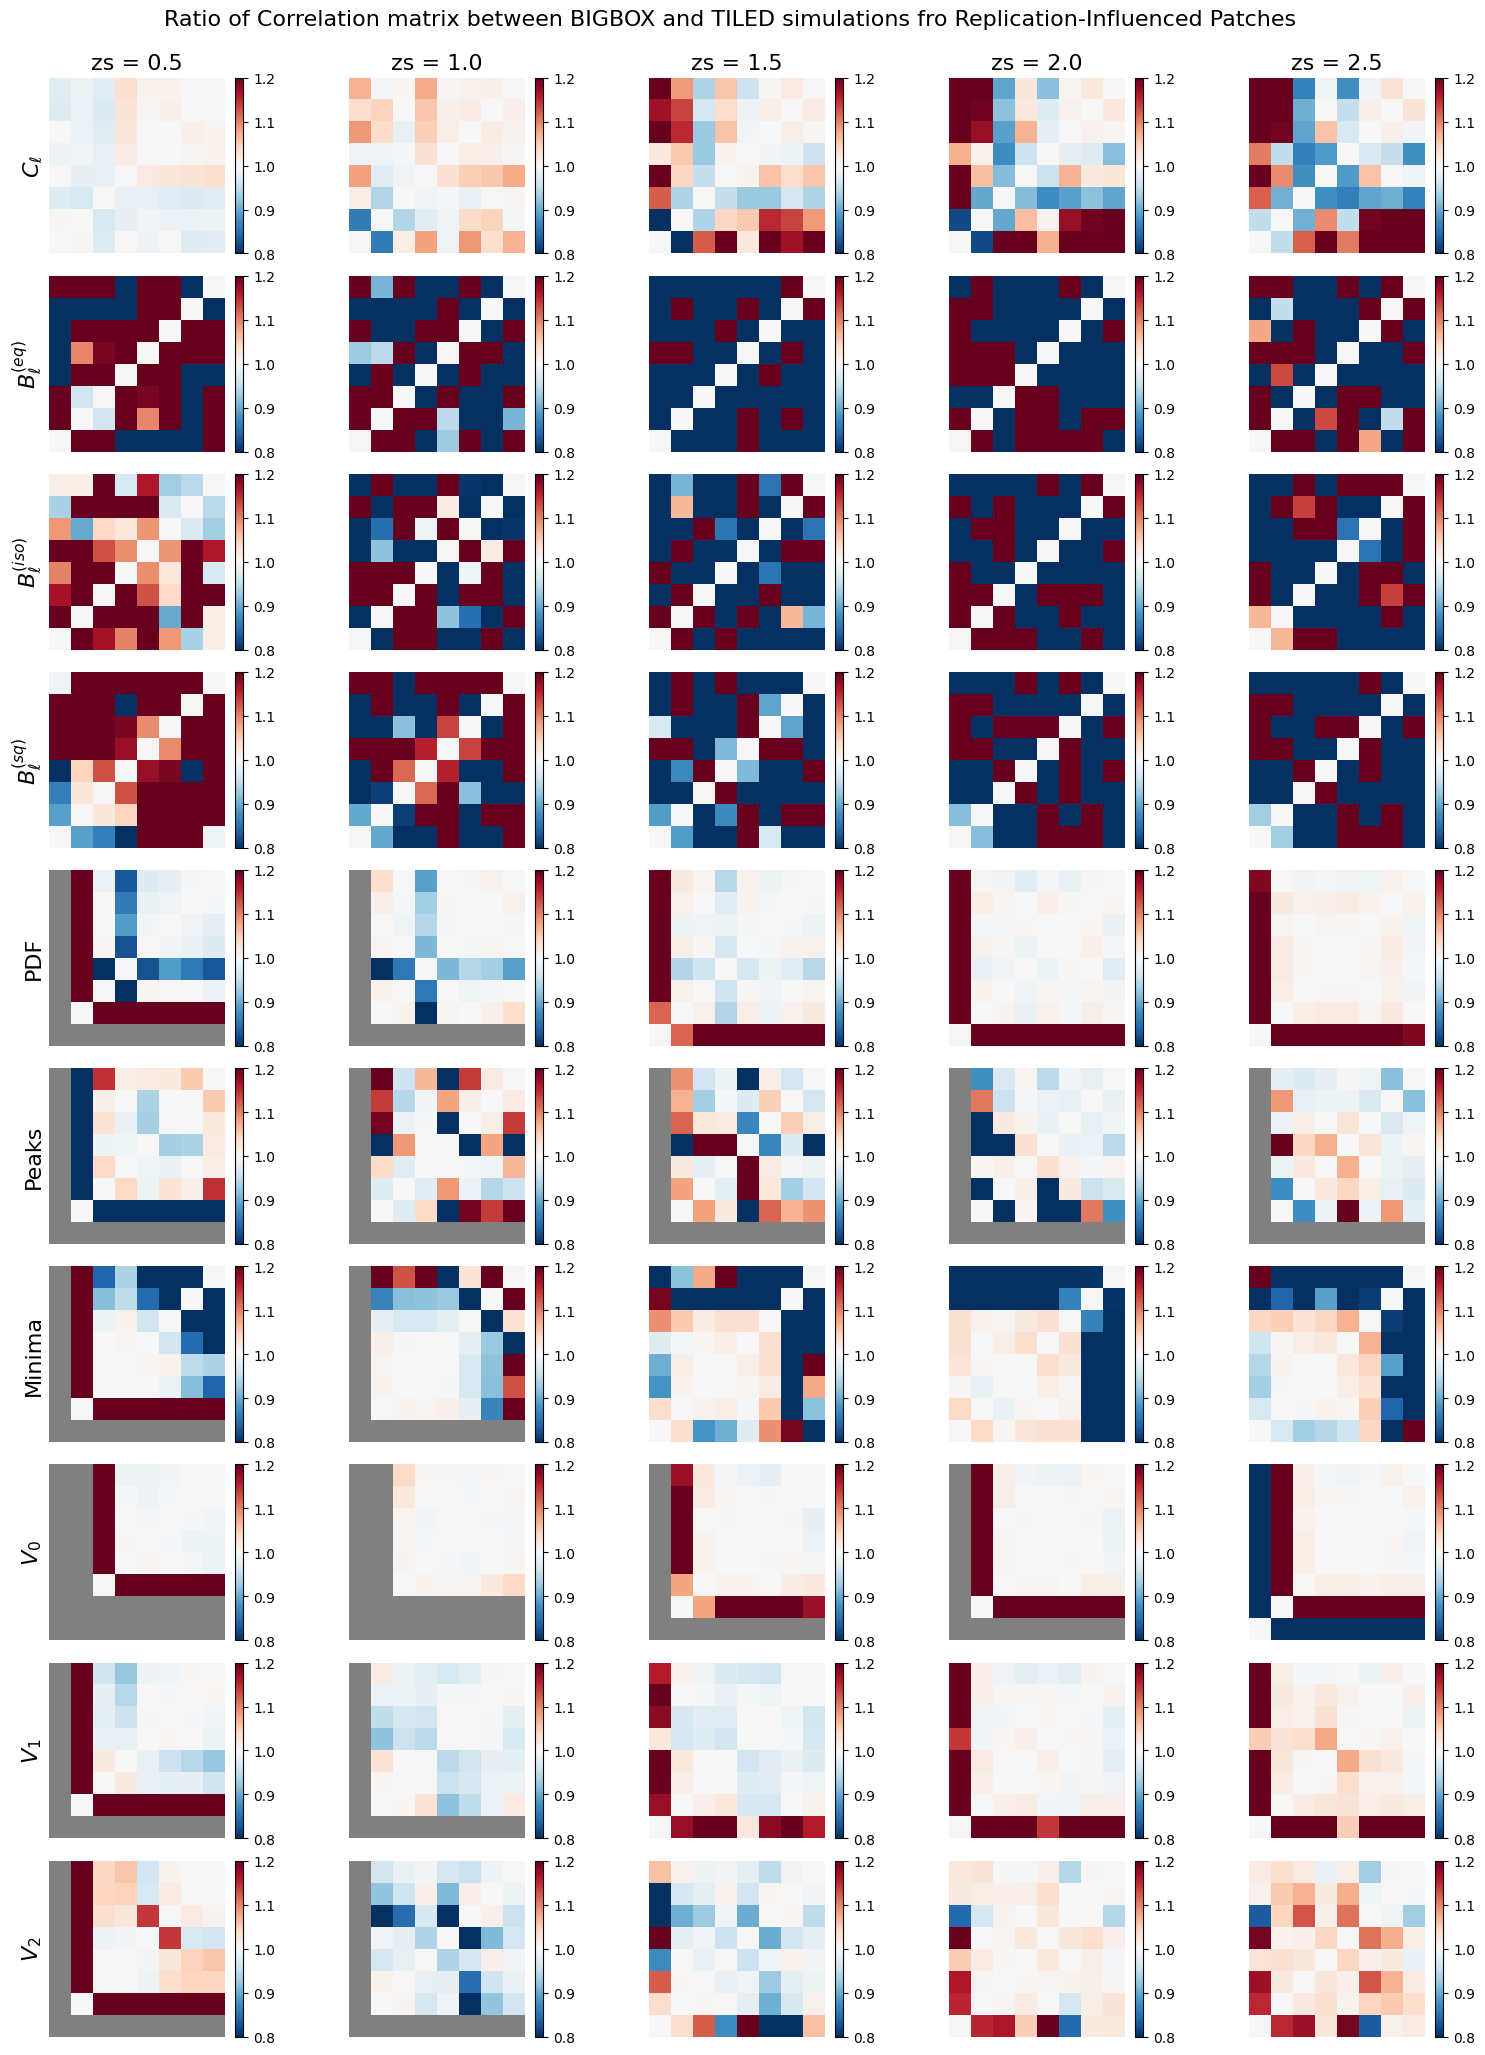
\includegraphics[width=\textwidth]{figures/results/corr_ratio_RIP.png}
    \caption[Correlation Ratios for RIP]{BIGBOX/TILED ratios of correlation matrices specifically for Replication-Influenced Patches (RIP). Similar to covariance ratios, RIP correlation ratios are consistently lower than those for RMPs. Off-diagonal structures differ from those in Figure~\ref{fig:corr_ratio_main} at lower redshifts but are likely to become more similar at higher redshifts.}
    \label{fig:boxreplication_corr_RIP}
\end{figure}

\clearpage